% Options for packages loaded elsewhere
% Options for packages loaded elsewhere
\PassOptionsToPackage{unicode}{hyperref}
\PassOptionsToPackage{hyphens}{url}
\PassOptionsToPackage{dvipsnames,svgnames,x11names}{xcolor}
%
\documentclass[
  12pt,
  letterpaper,
  DIV=11,
  numbers=noendperiod]{scrartcl}
\usepackage{xcolor}
\usepackage[margin=1in]{geometry}
\usepackage{amsmath,amssymb}
\setcounter{secnumdepth}{5}
\usepackage{iftex}
\ifPDFTeX
  \usepackage[T1]{fontenc}
  \usepackage[utf8]{inputenc}
  \usepackage{textcomp} % provide euro and other symbols
\else % if luatex or xetex
  \usepackage{unicode-math} % this also loads fontspec
  \defaultfontfeatures{Scale=MatchLowercase}
  \defaultfontfeatures[\rmfamily]{Ligatures=TeX,Scale=1}
\fi
\usepackage{lmodern}
\ifPDFTeX\else
  % xetex/luatex font selection
\fi
% Use upquote if available, for straight quotes in verbatim environments
\IfFileExists{upquote.sty}{\usepackage{upquote}}{}
\IfFileExists{microtype.sty}{% use microtype if available
  \usepackage[]{microtype}
  \UseMicrotypeSet[protrusion]{basicmath} % disable protrusion for tt fonts
}{}
\usepackage{setspace}
\makeatletter
\@ifundefined{KOMAClassName}{% if non-KOMA class
  \IfFileExists{parskip.sty}{%
    \usepackage{parskip}
  }{% else
    \setlength{\parindent}{0pt}
    \setlength{\parskip}{6pt plus 2pt minus 1pt}}
}{% if KOMA class
  \KOMAoptions{parskip=half}}
\makeatother
% Make \paragraph and \subparagraph free-standing
\makeatletter
\ifx\paragraph\undefined\else
  \let\oldparagraph\paragraph
  \renewcommand{\paragraph}{
    \@ifstar
      \xxxParagraphStar
      \xxxParagraphNoStar
  }
  \newcommand{\xxxParagraphStar}[1]{\oldparagraph*{#1}\mbox{}}
  \newcommand{\xxxParagraphNoStar}[1]{\oldparagraph{#1}\mbox{}}
\fi
\ifx\subparagraph\undefined\else
  \let\oldsubparagraph\subparagraph
  \renewcommand{\subparagraph}{
    \@ifstar
      \xxxSubParagraphStar
      \xxxSubParagraphNoStar
  }
  \newcommand{\xxxSubParagraphStar}[1]{\oldsubparagraph*{#1}\mbox{}}
  \newcommand{\xxxSubParagraphNoStar}[1]{\oldsubparagraph{#1}\mbox{}}
\fi
\makeatother


\usepackage{longtable,booktabs,array}
\usepackage{calc} % for calculating minipage widths
% Correct order of tables after \paragraph or \subparagraph
\usepackage{etoolbox}
\makeatletter
\patchcmd\longtable{\par}{\if@noskipsec\mbox{}\fi\par}{}{}
\makeatother
% Allow footnotes in longtable head/foot
\IfFileExists{footnotehyper.sty}{\usepackage{footnotehyper}}{\usepackage{footnote}}
\makesavenoteenv{longtable}
\usepackage{graphicx}
\makeatletter
\newsavebox\pandoc@box
\newcommand*\pandocbounded[1]{% scales image to fit in text height/width
  \sbox\pandoc@box{#1}%
  \Gscale@div\@tempa{\textheight}{\dimexpr\ht\pandoc@box+\dp\pandoc@box\relax}%
  \Gscale@div\@tempb{\linewidth}{\wd\pandoc@box}%
  \ifdim\@tempb\p@<\@tempa\p@\let\@tempa\@tempb\fi% select the smaller of both
  \ifdim\@tempa\p@<\p@\scalebox{\@tempa}{\usebox\pandoc@box}%
  \else\usebox{\pandoc@box}%
  \fi%
}
% Set default figure placement to htbp
\def\fps@figure{htbp}
\makeatother





\setlength{\emergencystretch}{3em} % prevent overfull lines

\providecommand{\tightlist}{%
  \setlength{\itemsep}{0pt}\setlength{\parskip}{0pt}}



 
\usepackage[backend=biber,style=apa,sorting=nyt,maxcitenames=2]{biblatex}
\addbibresource{../references/ce-library.bib}
\addbibresource{../references/sm-cited.bib}


\usepackage{xcolor}
\definecolor{linkblue}{HTML}{2E5EAA}
\definecolor{citegrey}{HTML}{4A4A4A}
\definecolor{urlblue}{HTML}{3A7CA5}
\usepackage{amsthm,amsmath,amsfonts,amssymb,float,caption,subcaption}
\usepackage{pdflscape}
\DeclareLanguageMapping{english}{english-apa}
\KOMAoption{captions}{tableheading}
\makeatletter
\@ifpackageloaded{caption}{}{\usepackage{caption}}
\AtBeginDocument{%
\ifdefined\contentsname
  \renewcommand*\contentsname{Table of contents}
\else
  \newcommand\contentsname{Table of contents}
\fi
\ifdefined\listfigurename
  \renewcommand*\listfigurename{List of Figures}
\else
  \newcommand\listfigurename{List of Figures}
\fi
\ifdefined\listtablename
  \renewcommand*\listtablename{List of Tables}
\else
  \newcommand\listtablename{List of Tables}
\fi
\ifdefined\figurename
  \renewcommand*\figurename{Figure}
\else
  \newcommand\figurename{Figure}
\fi
\ifdefined\tablename
  \renewcommand*\tablename{Table}
\else
  \newcommand\tablename{Table}
\fi
}
\@ifpackageloaded{float}{}{\usepackage{float}}
\floatstyle{ruled}
\@ifundefined{c@chapter}{\newfloat{codelisting}{h}{lop}}{\newfloat{codelisting}{h}{lop}[chapter]}
\floatname{codelisting}{Listing}
\newcommand*\listoflistings{\listof{codelisting}{List of Listings}}
\makeatother
\makeatletter
\makeatother
\makeatletter
\@ifpackageloaded{caption}{}{\usepackage{caption}}
\@ifpackageloaded{subcaption}{}{\usepackage{subcaption}}
\makeatother
\usepackage{bookmark}
\IfFileExists{xurl.sty}{\usepackage{xurl}}{} % add URL line breaks if available
\urlstyle{same}
\hypersetup{
  pdftitle={Quantifying Hidden Exploitation: Dual-Method Prevalence Estimates of Labour Exploitation among Domestic Workers in the United Kingdom},
  pdfauthor={Caroline Emberson; Scott Moser},
  colorlinks=true,
  linkcolor={linkblue},
  filecolor={Maroon},
  citecolor={BrickRed},
  urlcolor={urlblue},
  pdfcreator={LaTeX via pandoc}}


\title{Quantifying Hidden Exploitation: Dual-Method Prevalence Estimates
of Labour Exploitation among Domestic Workers in the United Kingdom}
\author{Caroline Emberson \and Scott Moser}
\date{11 July 2026}
\begin{document}
\maketitle
\begin{abstract}
Reliable indicators for SDG Target 8.7 are difficult to construct
because the populations most affected by labour exploitation are often
absent from standard household and labour-force surveys. This paper
develops a matched ego/alter survey design for measuring labour
exploitation among hidden populations. We apply respondent-driven
sampling and a network scale-up approach to the same survey instrument,
asking migrant domestic workers in the United Kingdom both about their
own experiences and about exploitation among domestic workers they know.
The design produces two complementary estimands: own-experience
prevalence and network-visible prevalence. We measure five ILO-aligned
indicators: excessive working hours, pay-related issues, limited access
to help, threats and abuse, and document withholding. We also construct
a formative composite risk index to capture gradations of exploitation
severity. In a civil-society-mediated web-RDS sample of 85 migrant
domestic workers, RDS-SS estimates indicate high own-experience
prevalence, while network scale-up estimates are substantially lower.
The divergence is consistent with a visibility gradient in which some
exploitation behaviours are more observable across peer networks than
others. The results should be interpreted as exploratory
population-adjusted estimates for an RDS-reachable population rather
than definitive national prevalence figures. The relative ordering of
prevalence of different forms of labour exploitation are robust across a
number of parameters. The paper contributes a replicable measurement
design for hidden-population social indicators relevant to SDG 8.7
monitoring.
\end{abstract}


\setstretch{1.15}
\section{Introduction}\label{sec-intro}

Modern slavery -- defined in UK law as an umbrella term which includes
slavery, servitude, forced labour, and human trafficking -- is named
under Sustainable Development Goal Target 8.7 as a priority for
elimination by 2030. Reliable prevalence measurement is a precondition
for monitoring that target, yet the populations most affected are
largely invisible to the household and labour-force surveys on which
official social indicators rely. Conventional household surveys
underestimate prevalence in this domain by an order of magnitude or
more, both because the populations affected (undocumented migrants,
live-in domestic workers, sex workers, agricultural day labourers) are
excluded from sampling frames, and because exploitation behaviours --
especially those at the more severe end of the spectrum -- are typically
not self-reported even when the respondent is contacted. The
civil-society and grey-literature evidence base on UK domestic workers
\autocite{kala08-new,serv23-closed} is qualitatively rich but does not
yield population-level prevalence estimates suitable for SDG monitoring
or comparison across populations. The International Labour
Organization's eleven indicators of forced labour
\autocite{ILO11-indicators,int25-ilo} provide an operational framework
for measuring modern slavery, but the empirical question of which
indicators are observable through which survey design remains open.
Studies typically apply one design -- household survey,
respondent-driven sampling (RDS), or the network scale-up method (NSUM)
-- and report prevalence accordingly. No prior study of modern-slavery
prevalence, to our knowledge, applies both RDS and NSUM to a single
matched survey instrument. Such a design would enable direct
triangulation of ego- and alter-based estimates on identical indicators
and, where they diverge, diagnostic inference about which exploitation
behaviours are visible across personal networks.

This paper makes two contributions. First, we apply RDS and NSUM to the
same survey instrument with the same respondents, eliciting ego-based
and alter-based estimates of an identical set of five ILO-aligned
indicators. The dual-method design produces two complementary estimands
(own-experience prevalence from RDS, network-visible prevalence from
NSUM); where they diverge, the gap itself is diagnostic evidence about
the visibility gradient of different exploitation behaviours within
workers' personal networks. Second, we treat modern slavery as a graded
phenomenon rather than a binary condition. The ILO's eleven indicators
of forced labour \autocite{ILO11-indicators,int25-ilo} anchor the
operational framework, and the ILO's survey-guidelines handbook
\autocite{hard24-ilo} distinguishes three `strong' indicators (retention
of identity documents, intimidation and threats, and physical and sexual
violence) --- any one of which is generally sufficient to identify
forced labour in survey settings --- from eight `medium' indicators,
several of which typically need to co-occur. The ordering supports both
indicator-level prevalence estimates and a composite risk index. Taken
together, the contribution of the paper is best read as developing and
demonstrating a defensible social-indicator measurement strategy for
hidden-population exploitation rather than as producing a definitive
national prevalence estimate. We demonstrate the strategy with a
respondent-driven sample of UK migrant domestic workers and discuss how
the methodology generalises to other hidden populations relevant to SDG
8.7 monitoring.

The remainder of the paper is organised as follows.
Section~\ref{sec-conceptualisation} conceptualises labour exploitation
as a graded formative indicator framework measured by five ILO-aligned
indicators arranged hierarchically by severity.
Section~\ref{sec-case-setting} describes the matched-instrument survey
design (Section~\ref{sec-study-design}) and the dual sampling approach
combining RDS and NSUM (Section~\ref{sec-survey-instrument}).
Section~\ref{sec-results} presents prevalence estimates by indicator and
method, including frequentist RDS-I/RDS-II/RDS-SS estimators
(Section~\ref{sec-descriptive}), Bayesian Model-Assisted inference
(Section~\ref{sec-composite-results}), and NSUM with sensitivity
analysis (Section~\ref{sec-binary-results}).
Section~\ref{sec-discussion} reads the RDS-NSUM divergence as diagnostic
evidence about visibility within workers' personal networks and
discusses implications for SDG 8.7 monitoring.

\section{Conceptualising Labour Exploitation and the Degree of
Risk}\label{sec-conceptualisation}

The International Labour Organization's eleven indicators of forced
labour \autocite{ILO11-indicators,int25-ilo} provide the canonical
operational framework for measuring modern slavery. The ILO's own
survey-guidelines handbook \autocite{hard24-ilo} distinguishes two
operational categories for use in forced-labour surveys: `strong'
indicators (intimidation and threats, physical and sexual violence,
retention of identity documents) any one of which is generally
sufficient on its own to identify a survey respondent as in forced
labour, and `medium' indicators (excessive overtime, wage withholding,
debt bondage, restriction of movement, isolation, abusive working and
living conditions, abuse of vulnerability, deception) whose evidentiary
weight for survey-based identification typically requires more than one
to be present. We adopt this severity ordering --- as it appears in the
ILO survey-guidelines handbook rather than the shorter
operational-indicators publications
\autocite{ILO11-indicators,int25-ilo}, which list the eleven without
ranking them --- to organise the reporting of the five binary indicators
below and to structure the reporting of the composite risk index. We
measure five indicators across the ordering, chosen to span the ILO
conceptual space efficiently within the constraints of a
matched-instrument ego/alter survey design. Three are medium indicators
-- excessive working hours, pay-related issues (combining wage
withholding with elements of debt bondage), and limited access to help
(combining restriction of movement with isolation, as both manifest in
the same observable behaviour in the domestic-work context). Two are
strong indicators -- threats and abuse (combining intimidation/threats
with physical and sexual violence, which prior qualitative work suggests
co-occur in this population: \textcite{yilm23-exploring}) and document
and passport withholding. The specific bundling of ILO indicators into
these five binary measures (e.g., combining intimidation/threats with
physical and sexual violence into a single `threats and abuse'
indicator) is our analytical choice, informed by the qualitative and
civil-society literature on UK migrant domestic workers
\autocite{kala08-new,mant16-modern,serv23-closed,yilm23-exploring}, not
a mapping the ILO itself publishes. The remaining two ILO indicators --
abuse of vulnerability and deception -- are not measured as standalone
binary prevalence indicators: both are too retrospective and judgemental
to elicit reliably through a brief survey of n=85 respondents (the
respondent would need to reconstruct intent and knowledge states from
the perspective of months or years after the fact). Both are nonetheless
included in the composite risk index (Appendix Table A.1, Categories 1
and 2; results in Section~\ref{sec-composite-results}). Where
appropriate we note this scope limitation in the discussion of results.

The composite risk index aggregates all eleven ILO indicators of forced
labour into a single continuous measure
(Section~\ref{sec-survey-instrument}, Table~\ref{tbl-indicator-mapping};
Appendix Table A.1 for per-category weights). It is constructed as a
formative additive composite: an individual is exposed to exploitation
if any of the indicators is present, and the indicators are constitutive
rather than reflective of an underlying severity. We conduct robustness
assessment by perturbing the weights
(Section~\ref{sec-weights-sensitivity}). Two further evidentiary
markers, NRM-referral history and payment below the national living
wage, are reported as separate binary flags and are not part of the
composite, as their direct evidentiary status under UK policy makes them
more useful read independently.

\subsection{Evaluating the Degree of Risk}\label{sec-degree-of-risk}

We conceptualise risk of labour exploitation from the workers'
perspective, spanning a spectrum from illegal employment practices
(below-minimum-wage payment, health and safety violations) through to
forced labour and modern slavery. The more ILO indicators present, the
stronger the likelihood of exploitation. We operationalise this in two
complementary ways: binary indicators classifying respondents as
exploited or not on each ILO-aligned dimension (threshold criteria,
Section~\ref{sec-binary-results}) and a continuous formative additive
composite risk index capturing gradations of vulnerability across all
eleven ILO indicators (Section~\ref{sec-composite-results}; the
Appendix, Section A, for full construction).

\section{Case Setting: Labour Exploitation Risk Among Transnational
Migrant Domestic Workers In The UK}\label{sec-case-setting}

Domestic work in the United Kingdom is performed predominantly by
transnational migrant women, the majority entering on tied Overseas
Domestic Worker (ODW) visas under which the right to remain is
conditional on employment with a specific employer
\autocite{mant16-modern,kala08-new,serv23-closed}. The combination of
tied immigration status, work performed inside the private home, and the
absence of routine workplace inspection creates structural conditions
under which labour exploitation can occur unobserved by employment
regulators, mainstream labour-market surveys, and the police
\autocite{romero_blueprint_2025}. Civil-society organisations
representing migrant domestic workers have documented patterns of wage
withholding, document confiscation, restricted movement, excessive
working hours, and threats and abuse over more than two decades
\autocite{kala08-new,mant16-modern,serv23-closed,yilm23-exploring}.
However, qualitative and case-based evidence have not yielded
population-level prevalence estimates suitable for SDG 8.7 monitoring or
cross-population comparison. The UK migrant domestic worker case is
therefore well-suited as the testbed for a measurement methodology aimed
at producing comparable prevalence indicators for hidden,
civil-society-mediated populations relevant to SDG 8.7 reporting. The
methodology demonstrated here generalises to other hidden populations
sharing the structural features of tied employment, private-home
workplaces, and civil-society-mediated access.

\subsection{Study Design and Sampling}\label{sec-study-design}

Respondent-Driven Sampling (RDS) is a network-based sampling method
designed to study hidden or hard-to-reach populations
\autocite{heck97-respondentdriven,heck11-comment,gile18-methods}. It
combines chain-referral sampling with a statistical framework to produce
population estimates that adjust for network structure and differential
recruitment probabilities. The method begins with a set of initial
participants (``seeds''), who recruit peers from their social networks.
Recruits, in turn, recruit others, creating waves of participation. The
number of each participant's recruits implicitly proxies for their
network degree (the number of eligible contacts they know), which is
used to adjust for selection bias--especially the oversampling of
high-degree individuals.

RDS has been widely used to sample hidden populations in public health
and social science research
\autocite{mccr12-evaluation,schw12-prevalence}, and network-based
referrals have been described as the only viable method to reach many
types of labour trafficking victims \autocite{zhang_measuring_2012}.
Recent applications include studies of exploitation among low-wage
workers in American cities \autocite{bern09-broken}, labour trafficking
in migrant communities \autocite{vinc17-estimating}, child labour in
India \autocite{zhan19-victims}, and commercial sexual exploitation in
Nepal \autocite{jord20-overcoming}.

Our approach can best be described as Web-based RDS
\autocite{wejn08-webbased}. We designed a web survey using the JISC
online survey interface, suitable for respondents to complete via mobile
phone. The main survey was conducted over five months between February
and July 2023.

\emph{Seed Selection and Recruitment}

We selected our first wave of participants nonrandomly by convenience
sampling. Mobile phone numbers were used both to identify seed
participants and to act as a unique identifier for those whom they
referred. To avoid sample homophily, original sample members were
selected from three distinct domestic worker communities facilitated by
civil society organisations. One was an exclusively online community of
transnational domestic workers working in the UK, the second represented
UK domestic workers of Filipino origin, and the third drew its
membership from the Latin American community of domestic workers, also
in the UK. Representatives from these organisations, along with other
academics with expertise in exploitation within domestic work,
contributed to survey question design and facilitated piloting of an
initial version of the survey, which was translated and made available
in four languages: English, Spanish, Tagalog, and Portuguese.

\emph{Incentive Design and Participation Verification}

A double incentive scheme rewarded respondents both for completing the
questionnaire and for each referral who went on to engage with the
survey. The challenge of incentive design is to set the incentive at a
level that adequately rewards respondents' time and participation, but
that also avoids the risk of fraudulent participation due to too high a
monetary gain \autocite{jord20-overcoming}. A sum of £10 was provided
for survey completion with a further £5 for each successful nomination.
While respondents were asked to nominate up to 10 domestic workers
within their existing social network, participation from up to five of
these was requested in subsequent waves. This approach is akin to the
use of vouchers in face-to-face studies as advocated by
\textcite{thompson_new_2020}.

Respondents were incentivised through lottery entry, consistent with the
design recommendations of the survey-incentive literature (full
literature review and incentive-design details in the Appendix, Section
D.7).

\subsection{Survey Instrument and
Indicators}\label{sec-survey-instrument}

The survey instrument was designed to capture both egocentric
(ego-based) and altercentric (alter-based) network information, enabling
the application of both RDS and NSUM estimation methods. Composite
measures to quantify the extent to which respondents were at risk of
labour exploitation, including severe forms of exploitation such as
forced labour, were constructed from existing exploitation typologies,
notably the ILO's Indicators of Forced Labour
\autocite{ILO11-indicators,int25-ilo} and the associated
survey-guidelines handbook \autocite{hard24-ilo}. The eleven ILO
indicators of forced labour \autocite{ILO11-indicators,int25-ilo}
provide the operational framework for our measurement strategy; the
medium/strong severity ordering used to organise the indicators follows
the ILO handbook on forced-labour surveys \autocite{hard24-ilo}.
Table~\ref{tbl-indicator-mapping} (below) maps each ILO indicator to its
measurement status in this paper: whether it is measured directly as a
binary prevalence indicator (reported in
Section~\ref{sec-binary-results}), whether it is included in the
formative additive composite risk index (reported in
Section~\ref{sec-composite-results}), and which survey questions elicit
the ego- and alter-based reports.

\begin{longtable}[]{@{}
  >{\raggedleft\arraybackslash}p{(\linewidth - 10\tabcolsep) * \real{0.0385}}
  >{\raggedright\arraybackslash}p{(\linewidth - 10\tabcolsep) * \real{0.3462}}
  >{\centering\arraybackslash}p{(\linewidth - 10\tabcolsep) * \real{0.1026}}
  >{\raggedright\arraybackslash}p{(\linewidth - 10\tabcolsep) * \real{0.2308}}
  >{\centering\arraybackslash}p{(\linewidth - 10\tabcolsep) * \real{0.1026}}
  >{\raggedright\arraybackslash}p{(\linewidth - 10\tabcolsep) * \real{0.1795}}@{}}
\caption{Mapping of the eleven ILO Indicators of Forced Labour to this
paper's measurement scheme. The five binary prevalence indicators
(right-hand grouping in column 4: document withholding, threats and
abuse, pay-related issues, limited access to help, excessive working
hours) jointly cover nine of the eleven ILO indicators (all except abuse
of vulnerability and deception, which are captured in the composite
only). The composite risk index covers all eleven ILO indicators through
eleven weighted sub-categories. Two further evidentiary markers --
NRM-referral history (Q80) and payment below the national living wage
(Q36) -- are reported as separate binary flags and are not part of the
composite. The medium/strong severity classification in column 2 follows
the ILO handbook on forced-labour surveys \autocite{hard24-ilo}; the
shorter operational-indicators publications
\autocite{ILO11-indicators,int25-ilo} list the eleven indicators without
publishing this severity ranking. Full per-category weight values are
given in Appendix Table A.1. Source: Authors' construction following ILO
\autocite*{ILO11-indicators,hard24-ilo,int25-ilo}.}\label{tbl-indicator-mapping}\tabularnewline
\toprule\noalign{}
\begin{minipage}[b]{\linewidth}\raggedleft
\#
\end{minipage} & \begin{minipage}[b]{\linewidth}\raggedright
ILO indicator (2012, 2017)
\end{minipage} & \begin{minipage}[b]{\linewidth}\centering
Severity
\end{minipage} & \begin{minipage}[b]{\linewidth}\raggedright
Binary indicator
\end{minipage} & \begin{minipage}[b]{\linewidth}\centering
Composite
\end{minipage} & \begin{minipage}[b]{\linewidth}\raggedright
Survey item(s)
\end{minipage} \\
\midrule\noalign{}
\endfirsthead
\toprule\noalign{}
\begin{minipage}[b]{\linewidth}\raggedleft
\#
\end{minipage} & \begin{minipage}[b]{\linewidth}\raggedright
ILO indicator (2012, 2017)
\end{minipage} & \begin{minipage}[b]{\linewidth}\centering
Severity
\end{minipage} & \begin{minipage}[b]{\linewidth}\raggedright
Binary indicator
\end{minipage} & \begin{minipage}[b]{\linewidth}\centering
Composite
\end{minipage} & \begin{minipage}[b]{\linewidth}\raggedright
Survey item(s)
\end{minipage} \\
\midrule\noalign{}
\endhead
\bottomrule\noalign{}
\endlastfoot
1 & Abuse of vulnerability & Medium & -- (composite only) & Cat 1 & Q29,
Q51 \\
2 & Deception & Medium & -- (composite only) & Cat 2 & Q45 \\
3 & Restriction of movement & Medium & Limited access to help & Cat 3 &
Q32, Q46 \\
4 & Isolation & Medium & Limited access to help & Cat 4 & Q65 \\
5 & Physical and sexual violence & Strong & Threats and abuse & Cat 5 &
Q44 (5c1, 5c1-b) \\
6 & Intimidation and threats & Strong & Threats and abuse & Cat 6 &
Q47 \\
7 & Retention of identity documents & Strong & Document withholding &
Cat 7 & Q70 \\
8 & Withholding of wages & Medium & Pay-related issues & Cat 8 & Q42 \\
9 & Debt bondage & Medium & Pay-related issues & Cat 9 & Q39 \\
10 & Abusive working and living conditions & Medium & Partial (Q48) &
Cat 10 & Q48, Q63, Q72, Q76 \\
11 & Excessive overtime & Medium & Excessive working hours & Cat 11 &
Q16, Q61, Q62 \\
\end{longtable}

Based on this mapping, we operationalise exploitation in two ways: (1)
five binary prevalence indicators classifying respondents as exploited
or not exploited on each dimension based on threshold criteria
(Section~\ref{sec-binary-results}), and (2) one continuous formative
additive composite risk index designed to capture gradations of
vulnerability across the full sample
(Section~\ref{sec-composite-results}).

Ego-based questions capture respondents' own experiences of exploitation
(used for RDS estimation), while alter-based questions ask respondents
to report on the exploitation experiences of domestic workers they know
(used for NSUM estimation). See the Appendix (Sections A and B) for
details of these survey questions and the construction of comparable
ego- and alter-based indicators.

\subsection{Sample Characteristics}\label{sec-sample-characteristics}

In total, we received completed online surveys from 97 respondents.
Twelve participants reported knowing zero domestic workers in the UK and
were excluded from RDS analysis because network degree information is
required for RDS weighting procedures. This resulted in an analytical
sample of 85 respondents for RDS-based estimation. Although the analytic
sample comprises 85 respondents, this is within the range used in
comparable respondent-driven sampling (RDS) and network scale-up (NSUM)
studies of hidden populations
\autocite{gile10-respondentdriven,goel10-assessing,gile11-improved}.
Statistical inference in these designs depends not on the absolute
sample size but on the structure of the recruitment network, degree
distribution, and convergence to equilibrium \autocite{salg04-sampling}.
Furthermore, model-assisted and Bayesian RDS estimators
\autocite{gile11-improved,gile18-methods} can produce model-assisted,
population-adjusted estimates under explicit assumptions, even in modest
samples, provided uncertainty and design limitations are made
transparent. In this study, we additionally employ a neighbourhood
bootstrap procedure that propagates sampling and network uncertainty,
providing robust confidence intervals consistent with small-sample
design-based inference \autocite{hand14-estimating}.

Of the 97 initial respondents, 90 identified themselves as transnational
migrants. In the analytical sample of \(n = 85\)
(Table~\ref{tbl-demographics}), 47\% regarded themselves as
self-employed, 37\% identified themselves as employees, and 17\%
categorised their employment status as agency workers. Filipino
respondents constitute the largest nationality cluster (65 respondents,
76\% of the analytical sample; Table~\ref{tbl-sample-chars} for the full
nationality × wave breakdown); other nationalities represented include
Dominican, Brazilian, Spanish, Colombian, Bolivian, Venezuelan, Cuban,
and Panamanian. Female domestic workers made up 98\% of the analytical
sample, with the remaining 2\% male. The age structure is skewed towards
older workers: 49\% of respondents are aged 45+, and a further 26\% are
aged 35--40 (Table~\ref{tbl-demographics}).

\begin{figure}[H]

\centering{

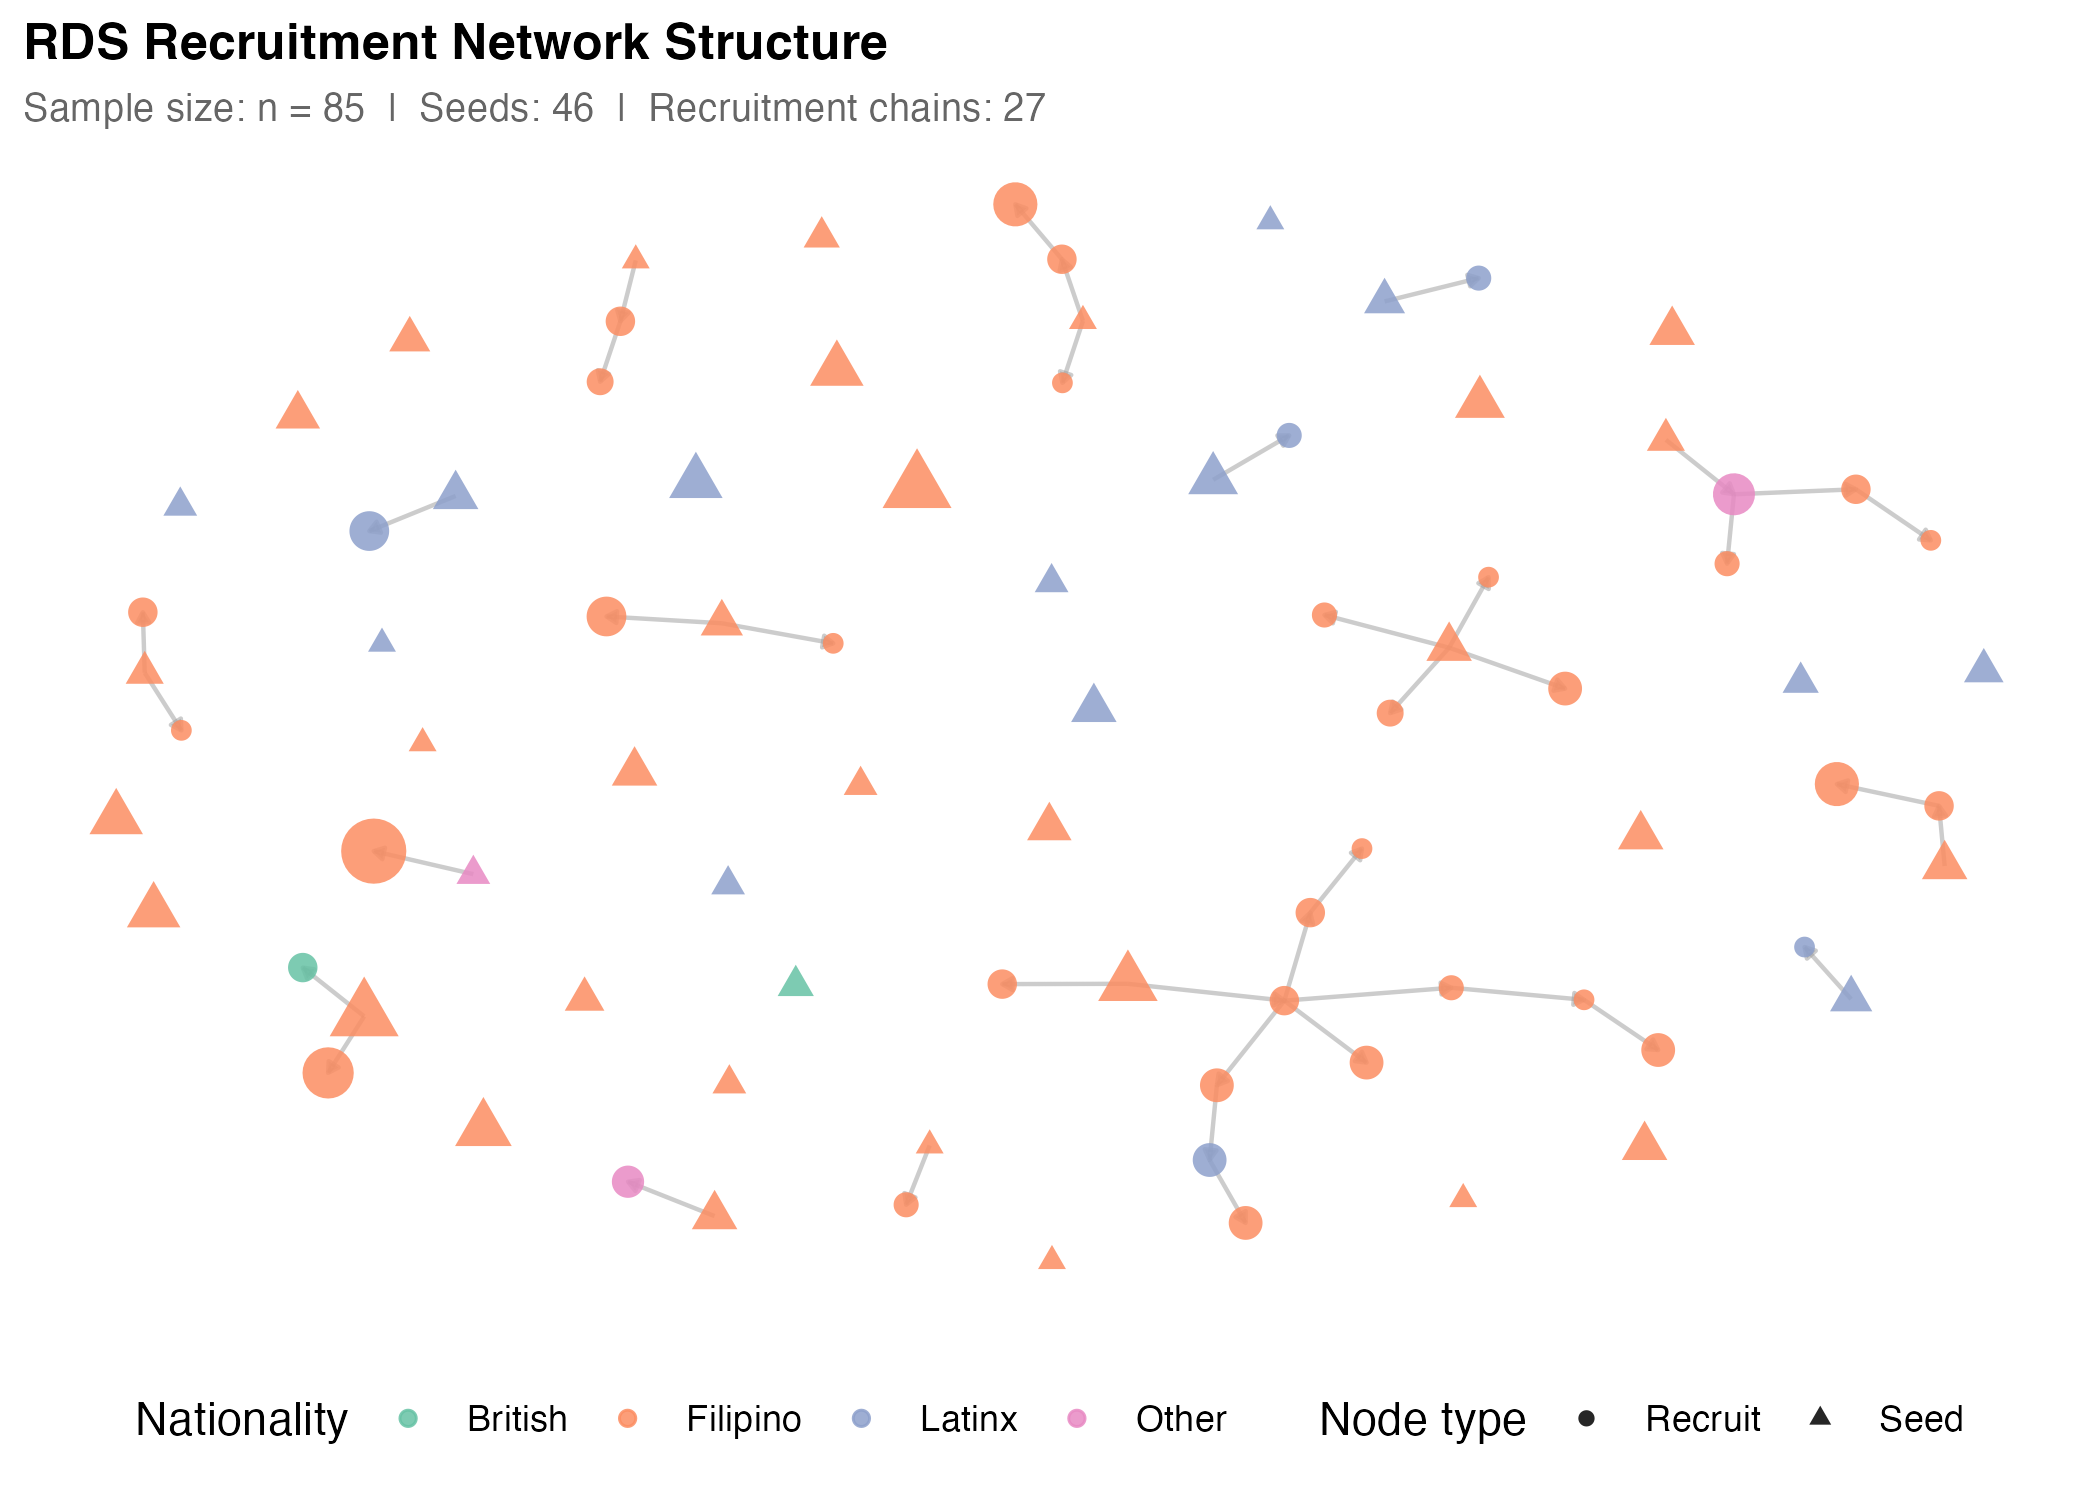
\includegraphics[width=6in,height=\textheight,keepaspectratio]{figures/fig1_recruitment_network.png}

}

\caption{\label{fig-recruitment}RDS Recruitment Network Structure.
Recruitment chains showing seed nodes (triangles) and recruit nodes
(circles). Node colours represent nationality clusters; node size is
proportional to network degree. Lines show recruiter-recruit
relationships. Source: Authors' own work.}

\end{figure}%

\begin{longtable}[]{@{}llrr@{}}
\caption{Sample demographics (n = 85 analytical sample). Response
categories for age and length of time in the UK follow the survey
codebook (Appendix A.3); the codebook's original response options
include a small ordinal gap between 40 and 45 years of age. Source:
Authors' construction from
\texttt{data/processed/prepared\_data.csv}.}\label{tbl-demographics}\tabularnewline
\toprule\noalign{}
Characteristic & Category & n & \% \\
\midrule\noalign{}
\endfirsthead
\toprule\noalign{}
Characteristic & Category & n & \% \\
\midrule\noalign{}
\endhead
\bottomrule\noalign{}
\endlastfoot
\textbf{Gender} & Female & 83 & 97.6\% \\
& Male & 2 & 2.4\% \\
\textbf{Age} & 23--25 & 1 & 1.2\% \\
& 26--35 & 20 & 23.5\% \\
& 35--40 & 22 & 25.9\% \\
& 45+ & 42 & 49.4\% \\
\textbf{Employment status} & Self-employed & 40 & 47.1\% \\
& Employee & 31 & 36.5\% \\
& Agency worker & 14 & 16.5\% \\
\textbf{Length of time in UK} & Less than 3 months & 3 & 3.5\% \\
& 3 months to 1 year & 19 & 22.4\% \\
& 1 to 3 years & 14 & 16.5\% \\
& More than 3 years & 49 & 57.6\% \\
\end{longtable}

\begin{longtable}[]{@{}
  >{\raggedright\arraybackslash}p{(\linewidth - 10\tabcolsep) * \real{0.2877}}
  >{\raggedleft\arraybackslash}p{(\linewidth - 10\tabcolsep) * \real{0.2192}}
  >{\raggedleft\arraybackslash}p{(\linewidth - 10\tabcolsep) * \real{0.1096}}
  >{\raggedleft\arraybackslash}p{(\linewidth - 10\tabcolsep) * \real{0.1096}}
  >{\raggedleft\arraybackslash}p{(\linewidth - 10\tabcolsep) * \real{0.1233}}
  >{\raggedleft\arraybackslash}p{(\linewidth - 10\tabcolsep) * \real{0.1507}}@{}}
\caption{Sample composition by nationality cluster and recruitment wave
(n = 85). Wave 0 indicates seed respondents; subsequent waves are
respondent-driven recruits. Filipino respondents dominate the sample
(76\%) and contribute the deepest recruitment chains; other nationality
clusters are smaller and shallower. Source: Authors' own
work.}\label{tbl-sample-chars}\tabularnewline
\toprule\noalign{}
\begin{minipage}[b]{\linewidth}\raggedright
Nationality cluster
\end{minipage} & \begin{minipage}[b]{\linewidth}\raggedleft
Wave 0 (seeds)
\end{minipage} & \begin{minipage}[b]{\linewidth}\raggedleft
Wave 1
\end{minipage} & \begin{minipage}[b]{\linewidth}\raggedleft
Wave 2
\end{minipage} & \begin{minipage}[b]{\linewidth}\raggedleft
Wave 3+
\end{minipage} & \begin{minipage}[b]{\linewidth}\raggedleft
Total (n)
\end{minipage} \\
\midrule\noalign{}
\endfirsthead
\toprule\noalign{}
\begin{minipage}[b]{\linewidth}\raggedright
Nationality cluster
\end{minipage} & \begin{minipage}[b]{\linewidth}\raggedleft
Wave 0 (seeds)
\end{minipage} & \begin{minipage}[b]{\linewidth}\raggedleft
Wave 1
\end{minipage} & \begin{minipage}[b]{\linewidth}\raggedleft
Wave 2
\end{minipage} & \begin{minipage}[b]{\linewidth}\raggedleft
Wave 3+
\end{minipage} & \begin{minipage}[b]{\linewidth}\raggedleft
Total (n)
\end{minipage} \\
\midrule\noalign{}
\endhead
\bottomrule\noalign{}
\endlastfoot
Filipino & 35 & 18 & 9 & 3 & 65 \\
Latinx & 4 & 2 & 0 & 0 & 6 \\
British & 2 & 0 & 0 & 0 & 2 \\
Other & 5 & 5 & 2 & 0 & 12 \\
\textbf{Total} & \textbf{46} & \textbf{25} & \textbf{11} & \textbf{3} &
\textbf{85} \\
\end{longtable}

\subsection{Estimation Framework}\label{sec-estimation-framework}

Before describing each estimator in turn, Table~\ref{tbl-estimands}
summarises the information each method uses, the population quantity
each method targets (its \emph{estimand}), and the principal source of
identification risk for each. The four estimators do not target the same
quantity. RDS-SS and MA-RDS estimate own-experience prevalence among the
RDS-reachable population of migrant domestic workers; NSUM estimates
network-visible prevalence among domestic-worker alters as reported by
the respondent; the composite risk index targets the RDS-adjusted mean
severity score. The order-of-magnitude RDS--NSUM gap should not be read
as two methods disagreeing about the same estimand. RDS estimates
own-experience prevalence, whereas NSUM estimates network-visible
prevalence among alters; the divergence is therefore substantively
interpretable rather than merely a discrepancy.

\begin{longtable}[]{@{}
  >{\raggedright\arraybackslash}p{(\linewidth - 6\tabcolsep) * \real{0.0960}}
  >{\raggedright\arraybackslash}p{(\linewidth - 6\tabcolsep) * \real{0.2778}}
  >{\raggedright\arraybackslash}p{(\linewidth - 6\tabcolsep) * \real{0.2980}}
  >{\raggedright\arraybackslash}p{(\linewidth - 6\tabcolsep) * \real{0.3283}}@{}}
\caption{Estimands and identification vulnerabilities of the four
estimators applied in this paper. Each row characterises one estimator:
what information from the survey it uses, what population quantity it
targets, and what the principal threat to identification is. Source:
Authors' construction.}\label{tbl-estimands}\tabularnewline
\toprule\noalign{}
\begin{minipage}[b]{\linewidth}\raggedright
Method
\end{minipage} & \begin{minipage}[b]{\linewidth}\raggedright
Information used
\end{minipage} & \begin{minipage}[b]{\linewidth}\raggedright
Estimand
\end{minipage} & \begin{minipage}[b]{\linewidth}\raggedright
Main vulnerability
\end{minipage} \\
\midrule\noalign{}
\endfirsthead
\toprule\noalign{}
\begin{minipage}[b]{\linewidth}\raggedright
Method
\end{minipage} & \begin{minipage}[b]{\linewidth}\raggedright
Information used
\end{minipage} & \begin{minipage}[b]{\linewidth}\raggedright
Estimand
\end{minipage} & \begin{minipage}[b]{\linewidth}\raggedright
Main vulnerability
\end{minipage} \\
\midrule\noalign{}
\endhead
\bottomrule\noalign{}
\endlastfoot
RDS-SS (binary, preferred) & Respondent's own experience + reported
degree + recruitment-chain structure & Own-experience prevalence among
the RDS-reachable population of UK migrant domestic workers & Seed
dependence, shallow recruitment chains, homophily, unobserved degree
heterogeneity \\
MA-RDS (supporting) & Same as RDS-SS, plus a working Exponential Random
Graph network model & Model-assisted own-experience prevalence (same
target as RDS-SS, with network-structure adjustment) & Network-model
misspecification, convergence limits at small \(n\); does not converge
on continuous outcomes \\
MBSU NSUM (binary, preferred) & Respondent reports about alters in their
personal network & Network-visible prevalence among domestic-worker
alters in the respondents' aggregated network & Transmission bias,
visibility gradient across exploitation behaviours, alter
misclassification, unknown true-positive rate (\(\tau\)) \\
Composite risk index & Respondent's own indicator profile across all
eleven ILO indicators & RDS-adjusted population mean of the
formative-additive severity score & Weight specification, construct
validity, formative-vs-reflective measurement assumptions \\
\end{longtable}

To the best of the authors' knowledge, the combined use of both methods
in the same study is rare in peer-reviewed academic research, though it
has appeared in government-funded reports and technical documents from
NGOs and research organizations
\autocite{ist20-prevalence,hick25-human}. This paper contributes to the
emerging methodological literature on combining RDS and NSUM in survey
research for hidden populations. We also developed a novel three-step
bootstrap procedure to address uncertainty in NSUM estimates.

\emph{RDS Estimation:} We implemented three RDS estimators, each with
distinct assumptions: RDS-I \autocite{salg04-sampling}, the
Volz--Heckathorn (VH) estimator \autocite{volz08-probability}, and
Gile's Successive Sampling (RDS-SS) estimator
\autocite{gile11-improved}. Given our small sample (85 respondents) and
non-negligible sampling fraction, RDS-SS serves as our primary estimator
for binary outcomes because it accounts for finite population effects.
RDS-I, which performs poorly in small samples and is highly sensitive to
seed dependence, is retained as a historical benchmark.

For continuous outcomes such as the exploitation risk index, we employ
Model-Assisted (MA-RDS) estimators \autocite{gile15-network}. MA-RDS is
design-based yet leverages a working Exponential Random Graph Model
(ERGM) with degree and homophily terms to approximate inclusion
probabilities conditional on observed seeds. This approach directly
addresses seed bias and homophily that conventional RDS estimators
cannot correct, accommodates finite-population effects through
successive-sampling logic, and supports valid estimation of both binary
and continuous outcomes. By conditioning on actual seed composition and
subgroup structure, the method reduces bias, improves efficiency, and
provides design-compatible bootstrap uncertainty
\autocite{gile11-improved}. We note one important limitation: the MA-RDS
implementation in the \texttt{RDS} package (\texttt{MA.estimates()}) is
designed primarily for binary traits, and we find that for the
continuous composite risk index it does not converge to a useful
posterior at our sample size (\(n=85\)); the credible interval covers
essentially the full support of the variable. We therefore report
frequentist RDS-SS estimates as the headline for the composite index and
reserve MA-RDS estimates for the five binary indicators (see
Section~\ref{sec-supporting-estimates} and the Appendix D.2).

\emph{Within-Population Scale-Up Estimation (NSUM):} We employ the
Modified Basic Scale-Up (MBSU) logic of \textcite{feeh16-generalizing}
in a non-standard, within-population configuration. In standard NSUM,
respondents are usually sampled from a frame population and report how
many people they know in a hidden population. Here, by contrast,
respondents are themselves UK migrant domestic workers and report on
other UK migrant domestic workers they know. We therefore treat the
design as a \emph{within-population scale-up} or \emph{alter-report
network prevalence} design: the target quantity is not the absolute size
of the hidden population, but the network-visible prevalence of
exploitation indicators among domestic-worker alters in respondents'
personal networks. This estimand differs from the standard NSUM estimand
and is documented in Table~\ref{tbl-estimands} above.

Let \(H_h\) denote the subset of domestic-worker alters who truly have
exploitation indicator \(h\), and let \(F\) denote the domestic-worker
alter universe induced by the survey's tie definition (the
\emph{frame}). For respondent \(i\), let \(y_{ih}\) be the reported
number of known domestic-worker alters with indicator \(h\), and let
\(d_i^{DW}\) be respondent \(i\)'s reported number of known UK migrant
domestic workers. The quantity \(d_i^{DW}\) is therefore a
domestic-worker alter degree: it is the denominator for the alter
reports \(y_{ih}\), not respondent \(i\)'s total personal network size
in the usual NSUM sense.

The unadjusted within-population NSUM estimator is

\begin{equation}\phantomsection\label{eq-1}{
\hat p_h^{NSUM} = \frac{\sum_i w_i y_{ih}}{\sum_i w_i d_i^{DW}},
}\end{equation}

where \(w_i\) is the RDS-derived survey weight. This estimator is a
weighted alter-level proportion: it estimates the share of reported
domestic-worker alters who are reported to have indicator \(h\). It
should therefore be interpreted as a measure of \emph{network-visible
prevalence} among domestic-worker alters, rather than as a direct
estimate of own-experience prevalence among respondents.

The MBSU-adjusted prevalence is then

\begin{equation}\phantomsection\label{eq-2}{
\hat p_h^{MBSU} =
\frac{1}{\delta_h \tau_h}
\frac{\sum_i w_i y_{ih}}{\sum_i w_i d_i^{DW}}.
}\end{equation}

Here, \(\delta_h\) is the indicator-specific within-population
degree-ratio adjustment: it captures whether domestic workers with
indicator \(h\) have, on average, more or fewer within-domestic-worker
network ties than domestic workers overall. Values of \(\delta_h < 1\)
imply that workers with indicator \(h\) are less connected within the
domestic-worker network and would therefore be under-represented in
alter reports. The parameter \(\tau_h\) is the indicator-specific
true-positive or visibility rate: the probability that an alter who
truly has indicator \(h\) is recognised and reported by the respondent
as having that indicator. Values of \(\tau_h < 1\) capture
under-reporting due to stigma, concealment, limited observability, or
social distance.

Because both the reporting frame and the alter universe are restricted
to domestic workers, \(\delta_h\) should not be read as a
general-population-to-hidden-population degree ratio. It is instead a
within-domestic-worker correction for differential network visibility of
workers with indicator \(h\). Similarly, \(\tau_h\) captures peer-tie
visibility for each exploitation indicator. This distinction is central
to the paper's visibility-gradient diagnostic: when RDS own-experience
estimates exceed NSUM alter-report estimates, the difference is
interpreted not simply as disagreement between methods, but as evidence
that some exploitation behaviours are less visible in peer networks than
others (Section~\ref{sec-divergence}).

Our headline NSUM result is the continuous-\(\tau\) sweep: for each
indicator, we report prevalence as a function of
\(\tau_h \in [0.40, 1.00]\), in increments of 0.05, with \(\delta_h\)
fixed at 0.9 and bootstrap 95\% confidence intervals at each value
(Appendix Figure D.4). For comparison with the discrete-tier NSUM
literature
\autocite{kill98-social,malt15-estimating,feeh16-generalizing}, we also
report three reference scenarios: Unadjusted
\((\delta_h = 1.0, \tau_h = 1.0\)), Moderate
\((\delta_h = 0.9, \tau_h = 0.85)\), and Conservative
\((\delta_h = 0.8, \tau_h = 0.70)\). These scenarios are presented as
reference points on the continuous sensitivity curve rather than as
separately identified estimates of \(\delta_h\) or \(\tau_h\).

\subsection{Comparative Rationale: Ego-Based vs.~Alter-Based
Inference}\label{sec-comparative-rationale}

RDS and NSUM both exploit social network structures but use
fundamentally different information for inference. RDS uses ego-based
information: respondents report their own characteristics and network
degree, which are combined with recruitment wave to adjust for unequal
inclusion probabilities. The underlying logic is that individuals with
larger networks are more likely to be recruited, creating bias toward
highly connected respondents. RDS estimators explicitly correct for this
by weighting observations according to network degree and recruitment
path.

NSUM uses alter-based information -- respondents serve as informants
about the wider hidden population, reporting how many people they know
with specific traits. These reports are scaled up using assumptions
about network size and visibility to infer prevalence in the broader
population. NSUM does not depend on recruitment chains but instead on
the accuracy of respondents' knowledge about others in their social
circles.

Applying both methods to the same dataset allows for triangulation
across two fundamentally different inferential logics--one anchored in
``who recruited whom'' (RDS), the other in ``how many alters fit this
category'' (NSUM).

\textbf{3.6 Choice of population size and the invariance of prevalence.}

For the prevalence estimates reported here, the assumed total
domestic-worker population size \(N\) either cancels algebraically or
has a negligible finite-population effect (related to \(n/N\) which is
negligable here) over the range of \(N\) values considered. RDS-I,
RDS-II/Volz-Heckathorn, and the MBSU NSUM prevalence formulas are
algebraically free of \(N\); RDS-SS and MA-RDS contain \(N\) only
through finite-population corrections whose magnitude scales with
\(n/N\). At \(n = 85\) our sampling fraction is at most 0.17\% (for
\(N = 50{,}000\)) and as low as 0.005\% (for \(N = 1{,}740{,}000\)), all
well below the conventional 5\% threshold at which finite-population
corrections become non-negligible. Headline estimates use
\(N = 980{,}000\) (the EU baseline); the MA-RDS Bayesian analysis uses
\(N = 50{,}000\) for computational tractability. Cached estimates across
all four values agree to within bootstrap noise; full algebraic
derivation and empirical confirmation are in the Appendix, Section D.1
(Population Size and the Invariance of Prevalence).

\subsection{Bootstrap and Sensitivity Procedures}\label{sec-bootstrap}

To appropriately characterise uncertainty in NSUM estimates, we
implement a three-step bootstrap procedure. This approach resamples
respondents, their reported alters, and the exploitation classifications
simultaneously, thereby capturing uncertainty at each stage of the
inference process. This procedure provides more realistic confidence
intervals than those generated by conventional variance estimators,
particularly for small samples such as ours. Details of the bootstrap
implementation and diagnostic checks are provided in the Appendix,
Section C. Several of the estimation procedures implemented here adopt
Bayesian or model-assisted frameworks, which are particularly
appropriate for modest sample sizes because they incorporate uncertainty
directly into the estimation process \autocite{gile18-methods}. Our
custom neighbourhood bootstrap procedure similarly quantifies
uncertainty by repeatedly resampling ego and alter information,
producing empirically grounded confidence intervals rather than relying
on asymptotic approximations that assume large samples.

For RDS estimators, we employ neighborhood bootstrap methods that
preserve the network structure while resampling
\autocite{yauc22-neighborhood}. Sensitivity analyses examine robustness
to population size assumptions (50K, 100K, 980K, 1.74M) and NSUM
adjustment factor values. Full results are reported in the Appendix.

\section{Results}\label{sec-results}

We present results in five subsections. Section~\ref{sec-descriptive}
describes the analytical sample. Sections
Section~\ref{sec-composite-results} and Section~\ref{sec-binary-results}
report the preferred prevalence estimates for the continuous composite
risk index and the five binary ILO-aligned indicators respectively. For
binary indicators, the preferred estimator is RDS-SS (Gile's Successive
Sampling) with neighbourhood-bootstrap 95\% confidence intervals; for
the composite risk index, also RDS-SS, because the Bayesian
Model-Assisted estimator does not converge to a useful posterior on
continuous outcomes at our sample size
(Section~\ref{sec-estimation-framework}). The preferred NSUM result is
the continuous-\(\tau\) sweep over \(\tau \in [0.40, 1.00]\) with
\(\delta\) fixed at 0.9 (Section~\ref{sec-sensitivity}; Appendix Figure
D.4); the Moderate discrete-tier point estimate (\(\delta = 0.9\),
\(\tau = 0.85\)) is reported alongside as a reference scenario for
direct comparison with the discrete-tier NSUM literature.
Section~\ref{sec-supporting-estimates} reports supporting estimates --
Bayesian Model-Assisted estimates for the five binary indicators,
alternative RDS estimators (RDS-I, RDS-II), and NSUM under alternative
adjustment-factor scenarios -- included for comparison and to support
the robustness claims in Section~\ref{sec-sensitivity}.
Section~\ref{sec-sensitivity} summarises the sensitivity analyses, with
full details in the Appendix.

The estimates reported below are exploratory population-adjusted
estimates for the RDS-reachable population of UK migrant domestic
workers connected to the participating civil-society networks (primarily
Kalayaan and the Latin American Women's Rights Service). They should not
be read as definitive national prevalence figures for all UK migrant
domestic workers. The reported quantities in Table~\ref{tbl-estimands}
target different population quantities
(Section~\ref{sec-estimation-framework}), so absolute levels also differ
by estimator in interpretable ways.

\subsection{Descriptive Overview}\label{sec-descriptive}

Sample demographics are presented in Table~\ref{tbl-demographics};
sample composition by nationality cluster and recruitment wave in
Table~\ref{tbl-sample-chars}; the recruitment network in
Figure~\ref{fig-recruitment}. 97 respondents completed the survey; 85
with non-zero network degree were included in RDS analysis. The
analytical sample is 93\% transnational migrant, 98\% female, 76\%
Filipino, with 49\% aged 45+ and 47\% self-employed.

\subsubsection{RDS Sampling Diagnostics}\label{sec-rds-diagnostics}

Because the RDS estimators reported below rely on assumptions about
chain propagation, degree homogeneity within seed groups, and reaching
equilibrium across recruitment waves, we report the key sampling
diagnostics here in the main text rather than in the supplement. The
diagnostics are summarised in Table~\ref{tbl-rds-diagnostics} and
visualised in Figure~\ref{fig-rds-diagnostics};
Figure~\ref{fig-recruitment} (above) shows the full recruitment graph.

\begin{longtable}[]{@{}
  >{\raggedright\arraybackslash}p{(\linewidth - 0\tabcolsep) * \real{1.0096}}@{}}
\caption{RDS sampling diagnostics for the analytical sample (n = 85).
Computed from the anonymised processed analysis dataset; replication
code is available in the OSF repository. See
Section~\ref{sec-rds-diagnostics} below and the Appendix (Section D) for
the full set. Source: Authors'
construction.}\label{tbl-rds-diagnostics}\tabularnewline
\toprule\noalign{}
\begin{minipage}[b]{\linewidth}\raggedright
Diagnostic \textbar{} Value \textbar{} Interpretation
\end{minipage} \\
\midrule\noalign{}
\endfirsthead
\toprule\noalign{}
\begin{minipage}[b]{\linewidth}\raggedright
Diagnostic \textbar{} Value \textbar{} Interpretation
\end{minipage} \\
\midrule\noalign{}
\endhead
\bottomrule\noalign{}
\endlastfoot
\end{longtable}

\begin{figure}[H]

\centering{

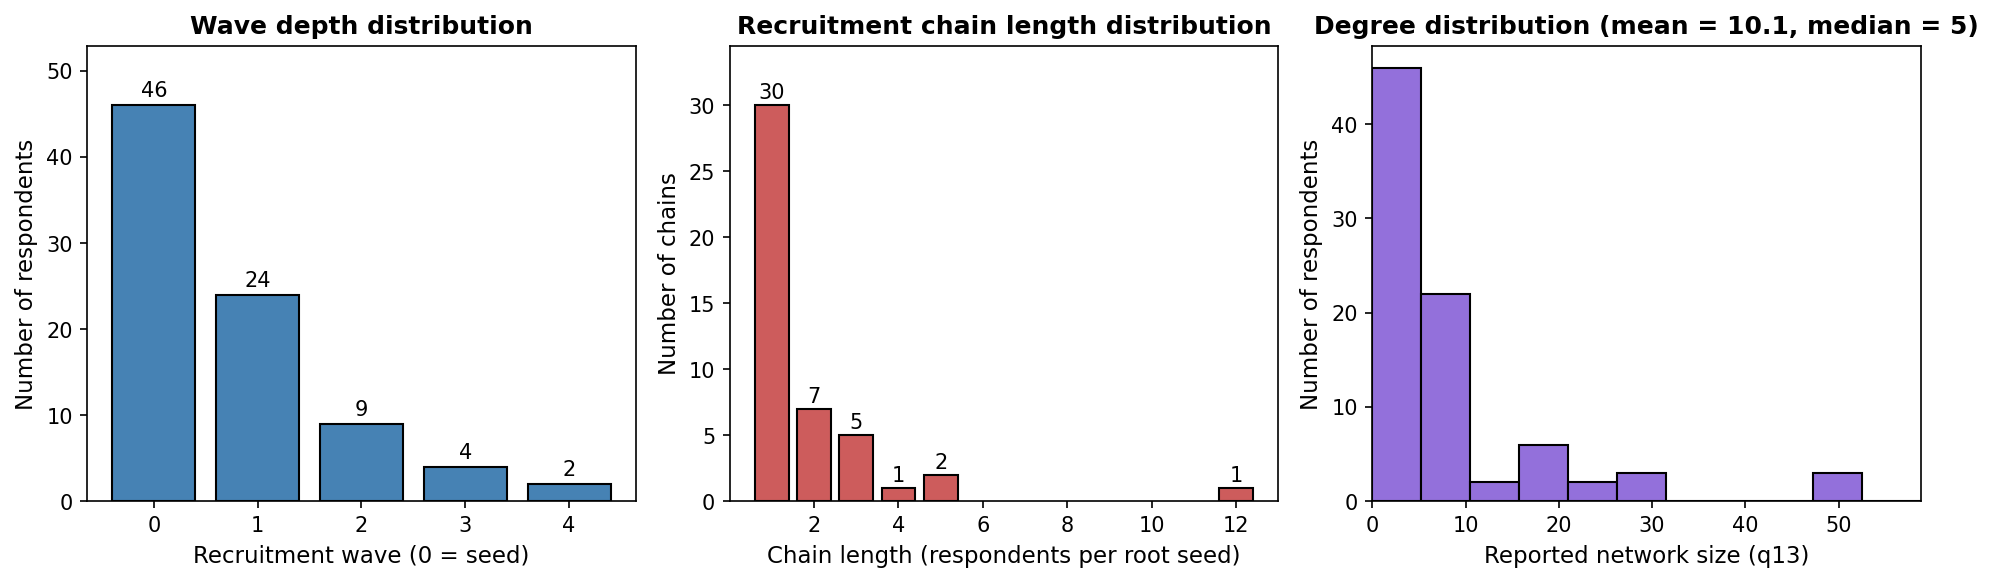
\includegraphics[width=6in,height=\textheight,keepaspectratio]{figures/rds_diagnostics.png}

}

\caption{\label{fig-rds-diagnostics}RDS sampling-design diagnostics.
Left: distribution of respondents by recruitment wave; majority are
seeds (wave 0) with only 6 of 85 respondents reaching wave 3 or higher.
Middle: distribution of recruitment-chain lengths by root seed; 30 of 46
chains are singletons (seed with no recruits), and one chain (seed \#55,
length 12) accounts for a disproportionate share of wave-2+ respondents.
Right: distribution of reported network size (q13), showing strong right
skew (median 5, mean 8.9, max 105). Source: Authors' construction.
Computed from the anonymised processed analysis dataset; replication
code is available in the OSF repository.}

\end{figure}%

Three features warrant acknowledgement. The high share of seeds (54\%)
and low share of wave-3+ respondents (7\%) mean the sample is closer to
a \emph{civil-society-mediated web-RDS sample with network adjustment}
than to a fully propagated RDS sample; the standard RDS assumption of
approximately stationary sampling distribution is therefore only
partially satisfied. The chain-length distribution is also highly
skewed: one chain (seed \#55, length 12) accounts for roughly a third of
wave-2+ respondents, and a leave-one-out sensitivity excluding that
chain (reported in Appendix Section D.8) does not change the rank
ordering of indicators. Finally, with 76\% of the sample Filipino, most
chains are within-Filipino, so prevalence estimates are best read as
estimates for the Filipino-dominated civil-society-reachable
subpopulation rather than for all UK migrant domestic workers. The
practical implication for the headline numbers is that RDS-SS, MA-RDS,
and the composite index should all be read with this constrained
sampling structure in view; the RDS-I vs RDS-SS comparison reported in
Section~\ref{sec-supporting-estimates} quantifies how much the standard
equilibrium assumption matters (RDS-I runs 5--15 percentage points
higher, with the gap larger where seed-cluster homophily is strongest).

\subsection{Continuous Risk Index: RDS-SS
Estimates}\label{sec-composite-results}

One of the central contributions of this study is the introduction of a
continuous risk index measuring degree of exposure to labour
exploitation. The index is constructed from all eleven ILO indicators of
forced labour. Each of the eleven ILO indicator categories contributes
equally to the composite (maximum 0.09 per category, giving a total
maximum score of 0.99); within a category, weight is distributed evenly
across the sub-questions used to code it. The composite is therefore
uniform-weighted at the ILO-category level and does not itself impose
the medium/strong severity ordering, though we use that ordering
(Section 2) to organise reporting and interpretation. The
weight-perturbation robustness check reported in
Section~\ref{sec-weights-sensitivity} confirms that the ranking of
respondents by composite risk is essentially invariant to the specific
weight choice. NRM-referral history and payment below the national
living wage are reported as separate binary evidentiary flags and are
not part of the composite (Section~\ref{sec-survey-instrument},
Table~\ref{tbl-indicator-mapping}; full per-category weights in Appendix
Table A.1). Rather than treating exploitation as a dichotomy, the risk
index conceptualises every domestic worker as facing some degree of
potential exploitation, varying continuously in intensity from low to
high.

The preferred population-adjusted estimate uses Gile's Successive
Sampling (RDS-SS) Horvitz-Thompson estimator with neighbourhood
bootstrap. The estimated mean risk index for the RDS-reachable
population of UK migrant domestic workers connected to the participating
civil-society networks is 37.0\% of the theoretical maximum (95\% CI
30.9--44.0\%), very close to the observed sample mean of 37.5\% --
indicating that the RDS-SS finite-population adjustment makes only a
small correction at our sampling fraction. We report RDS-SS rather than
the Bayesian Model-Assisted estimator for the composite index because,
as noted in Section~\ref{sec-estimation-framework}, MA-RDS does not
converge to a useful posterior on continuous traits at this sample size;
for completeness Figure~\ref{fig-composite} shows the MA estimate
alongside the RDS-SS and sample estimates, with the wide MA credible
interval making the limitation visible.

\begin{figure}[H]

\centering{

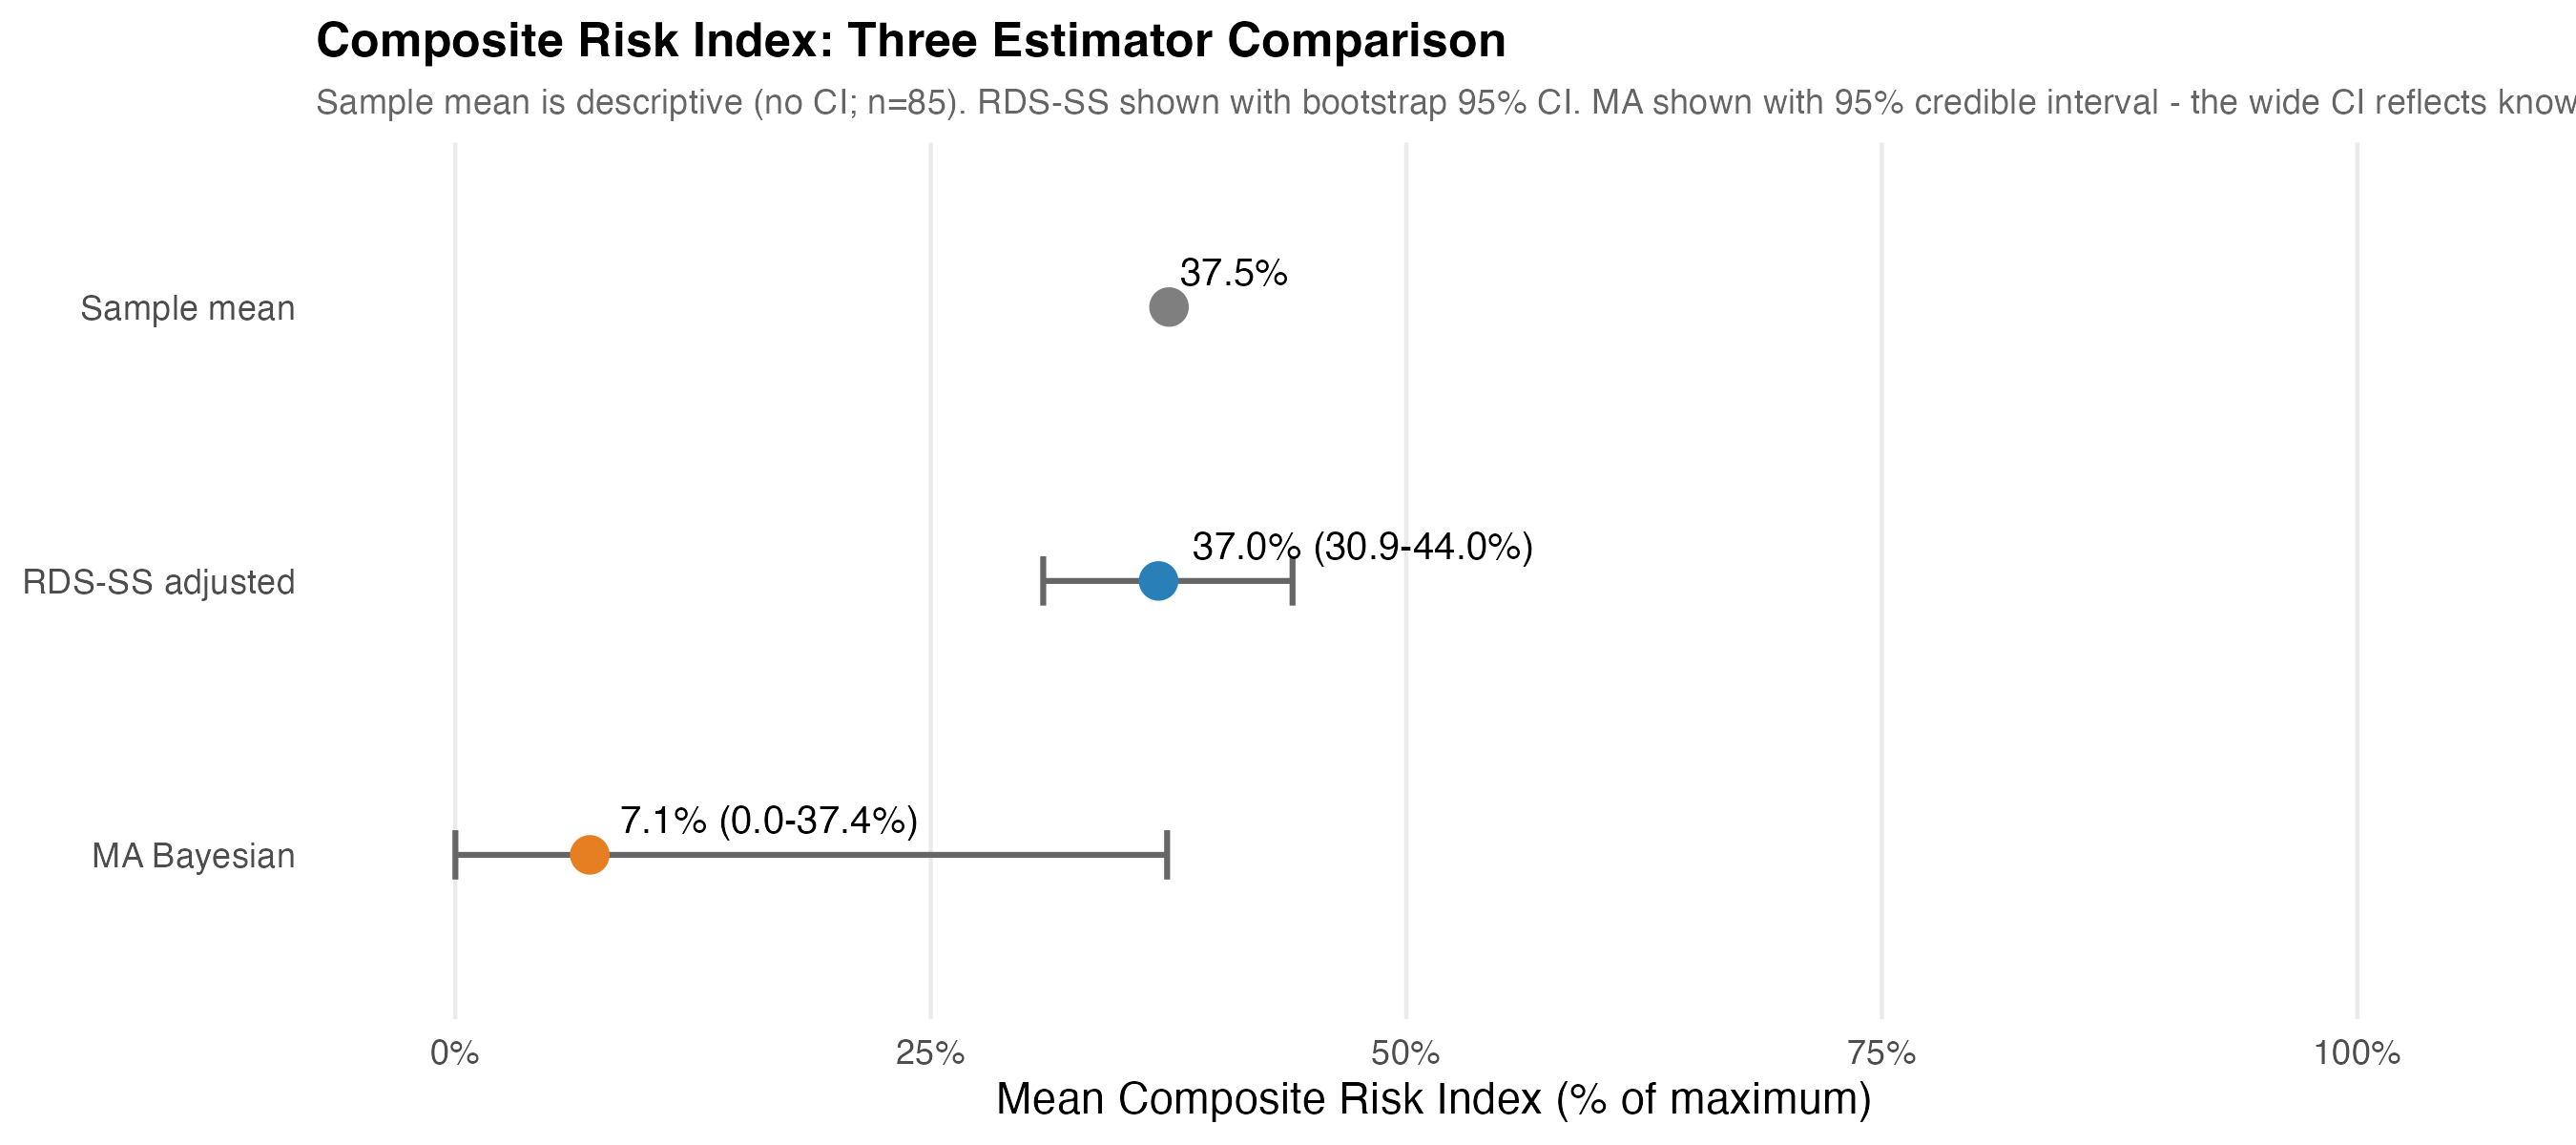
\includegraphics[width=6in,height=\textheight,keepaspectratio]{figures/fig3_composite_risk.png}

}

\caption{\label{fig-composite}Composite Risk Index: Comparison of Three
Estimators. Mean composite risk index across the observed RDS sample
(descriptive; n=85), the RDS-SS adjusted estimator (Gile's Successive
Sampling with bootstrap 95\% CI), and the Bayesian Model-Assisted (MA)
estimator (with 95\% credible interval). The wide MA credible interval
reflects known limitations of model-assisted inference for continuous
outcomes; the RDS-SS estimate is the more reliable population-adjusted
figure. Source: Authors' own work.}

\end{figure}%

\subsection{Binary Exploitation Indicators: Preferred Prevalence
Estimates}\label{sec-binary-results}

Table~\ref{tbl-preferred-estimates} reports the preferred prevalence
estimates for each of the five binary ILO-aligned indicators in the
RDS-reachable population, presenting RDS-SS (ego-based) and MBSU NSUM
Moderate (alter-based) estimates side by side. Appendix Figure D.2 shows
the RDS-SS and RDS-I estimates with per-method bootstrap CIs for visual
comparison (the preferred binary-indicator estimator is RDS-SS).

Prevalence is high for most indicators in this hidden population. RDS-SS
estimates range from 35.4\% for document withholding to 84.2\% for
excessive working hours; MBSU Moderate NSUM estimates range from 1.08\%
(document withholding) to 2.98\% (excessive hours). The
order-of-magnitude difference between RDS and NSUM is consistent with a
visibility gradient: ego-based RDS reports capture what the respondent
personally experienced, alter-based NSUM reports capture what other
domestic workers can see. For behaviours that occur behind closed doors,
the gap between own-experience and network-visible reports is large, and
the divergence between RDS and NSUM estimates is correspondingly large
(Section~\ref{sec-divergence} develops the diagnostic interpretation in
detail; the gap also reflects differences in estimand, sampling frame,
transmission bias, and the unknown true-positive rate). Within methods,
the ordering of indicators by prevalence is remarkably stable: excessive
working hours consistently the highest, followed by threats and abuse
and pay-related issues, with document withholding the lowest. This
consistency across methods, even where absolute levels differ, is a
robustness signal for the ordering of the indicators.

\begin{longtable}[]{@{}
  >{\raggedright\arraybackslash}p{(\linewidth - 4\tabcolsep) * \real{0.3091}}
  >{\raggedright\arraybackslash}p{(\linewidth - 4\tabcolsep) * \real{0.2545}}
  >{\raggedright\arraybackslash}p{(\linewidth - 4\tabcolsep) * \real{0.4364}}@{}}
\caption{Preferred prevalence estimates for the five binary ILO-aligned
indicators (UK migrant domestic workers connected to participating
civil-society networks; \(N\) = 980,000 assumed for absolute counts).
RDS-SS columns from neighbourhood-bootstrap 95\% CIs (\(B\) = 1000);
MBSU NSUM (Moderate: \(\delta\) = 0.9, \(\tau\) = 0.85) columns from
neighbourhood-bootstrap 95\% CIs. Source: Authors' own
work.}\label{tbl-preferred-estimates}\tabularnewline
\toprule\noalign{}
\begin{minipage}[b]{\linewidth}\raggedright
\textbf{Indicator}
\end{minipage} & \begin{minipage}[b]{\linewidth}\raggedright
\textbf{RDS-SS (95\% CI)}
\end{minipage} & \begin{minipage}[b]{\linewidth}\raggedright
\textbf{MBSU NSUM (Moderate) (95\% CI)}
\end{minipage} \\
\midrule\noalign{}
\endfirsthead
\toprule\noalign{}
\begin{minipage}[b]{\linewidth}\raggedright
\textbf{Indicator}
\end{minipage} & \begin{minipage}[b]{\linewidth}\raggedright
\textbf{RDS-SS (95\% CI)}
\end{minipage} & \begin{minipage}[b]{\linewidth}\raggedright
\textbf{MBSU NSUM (Moderate) (95\% CI)}
\end{minipage} \\
\midrule\noalign{}
\endhead
\bottomrule\noalign{}
\endlastfoot
Document withholding & 35.4\% (21.1--49.8\%) & 1.08\% (0.30--3.13\%) \\
Threats and abuse & 56.9\% (42.3--72.1\%) & 2.69\% (1.86--5.86\%) \\
Pay-related issues & 51.6\% (36.5--65.5\%) & 2.88\% (1.90--5.68\%) \\
Excessive working hours & 84.2\% (72.2--93.6\%) & 2.98\%
(1.84--5.51\%) \\
Limited access to help & 60.6\% (45.2--74.1\%) & 2.03\%
(0.67--4.88\%) \\
\end{longtable}

\begin{figure}[H]

\centering{

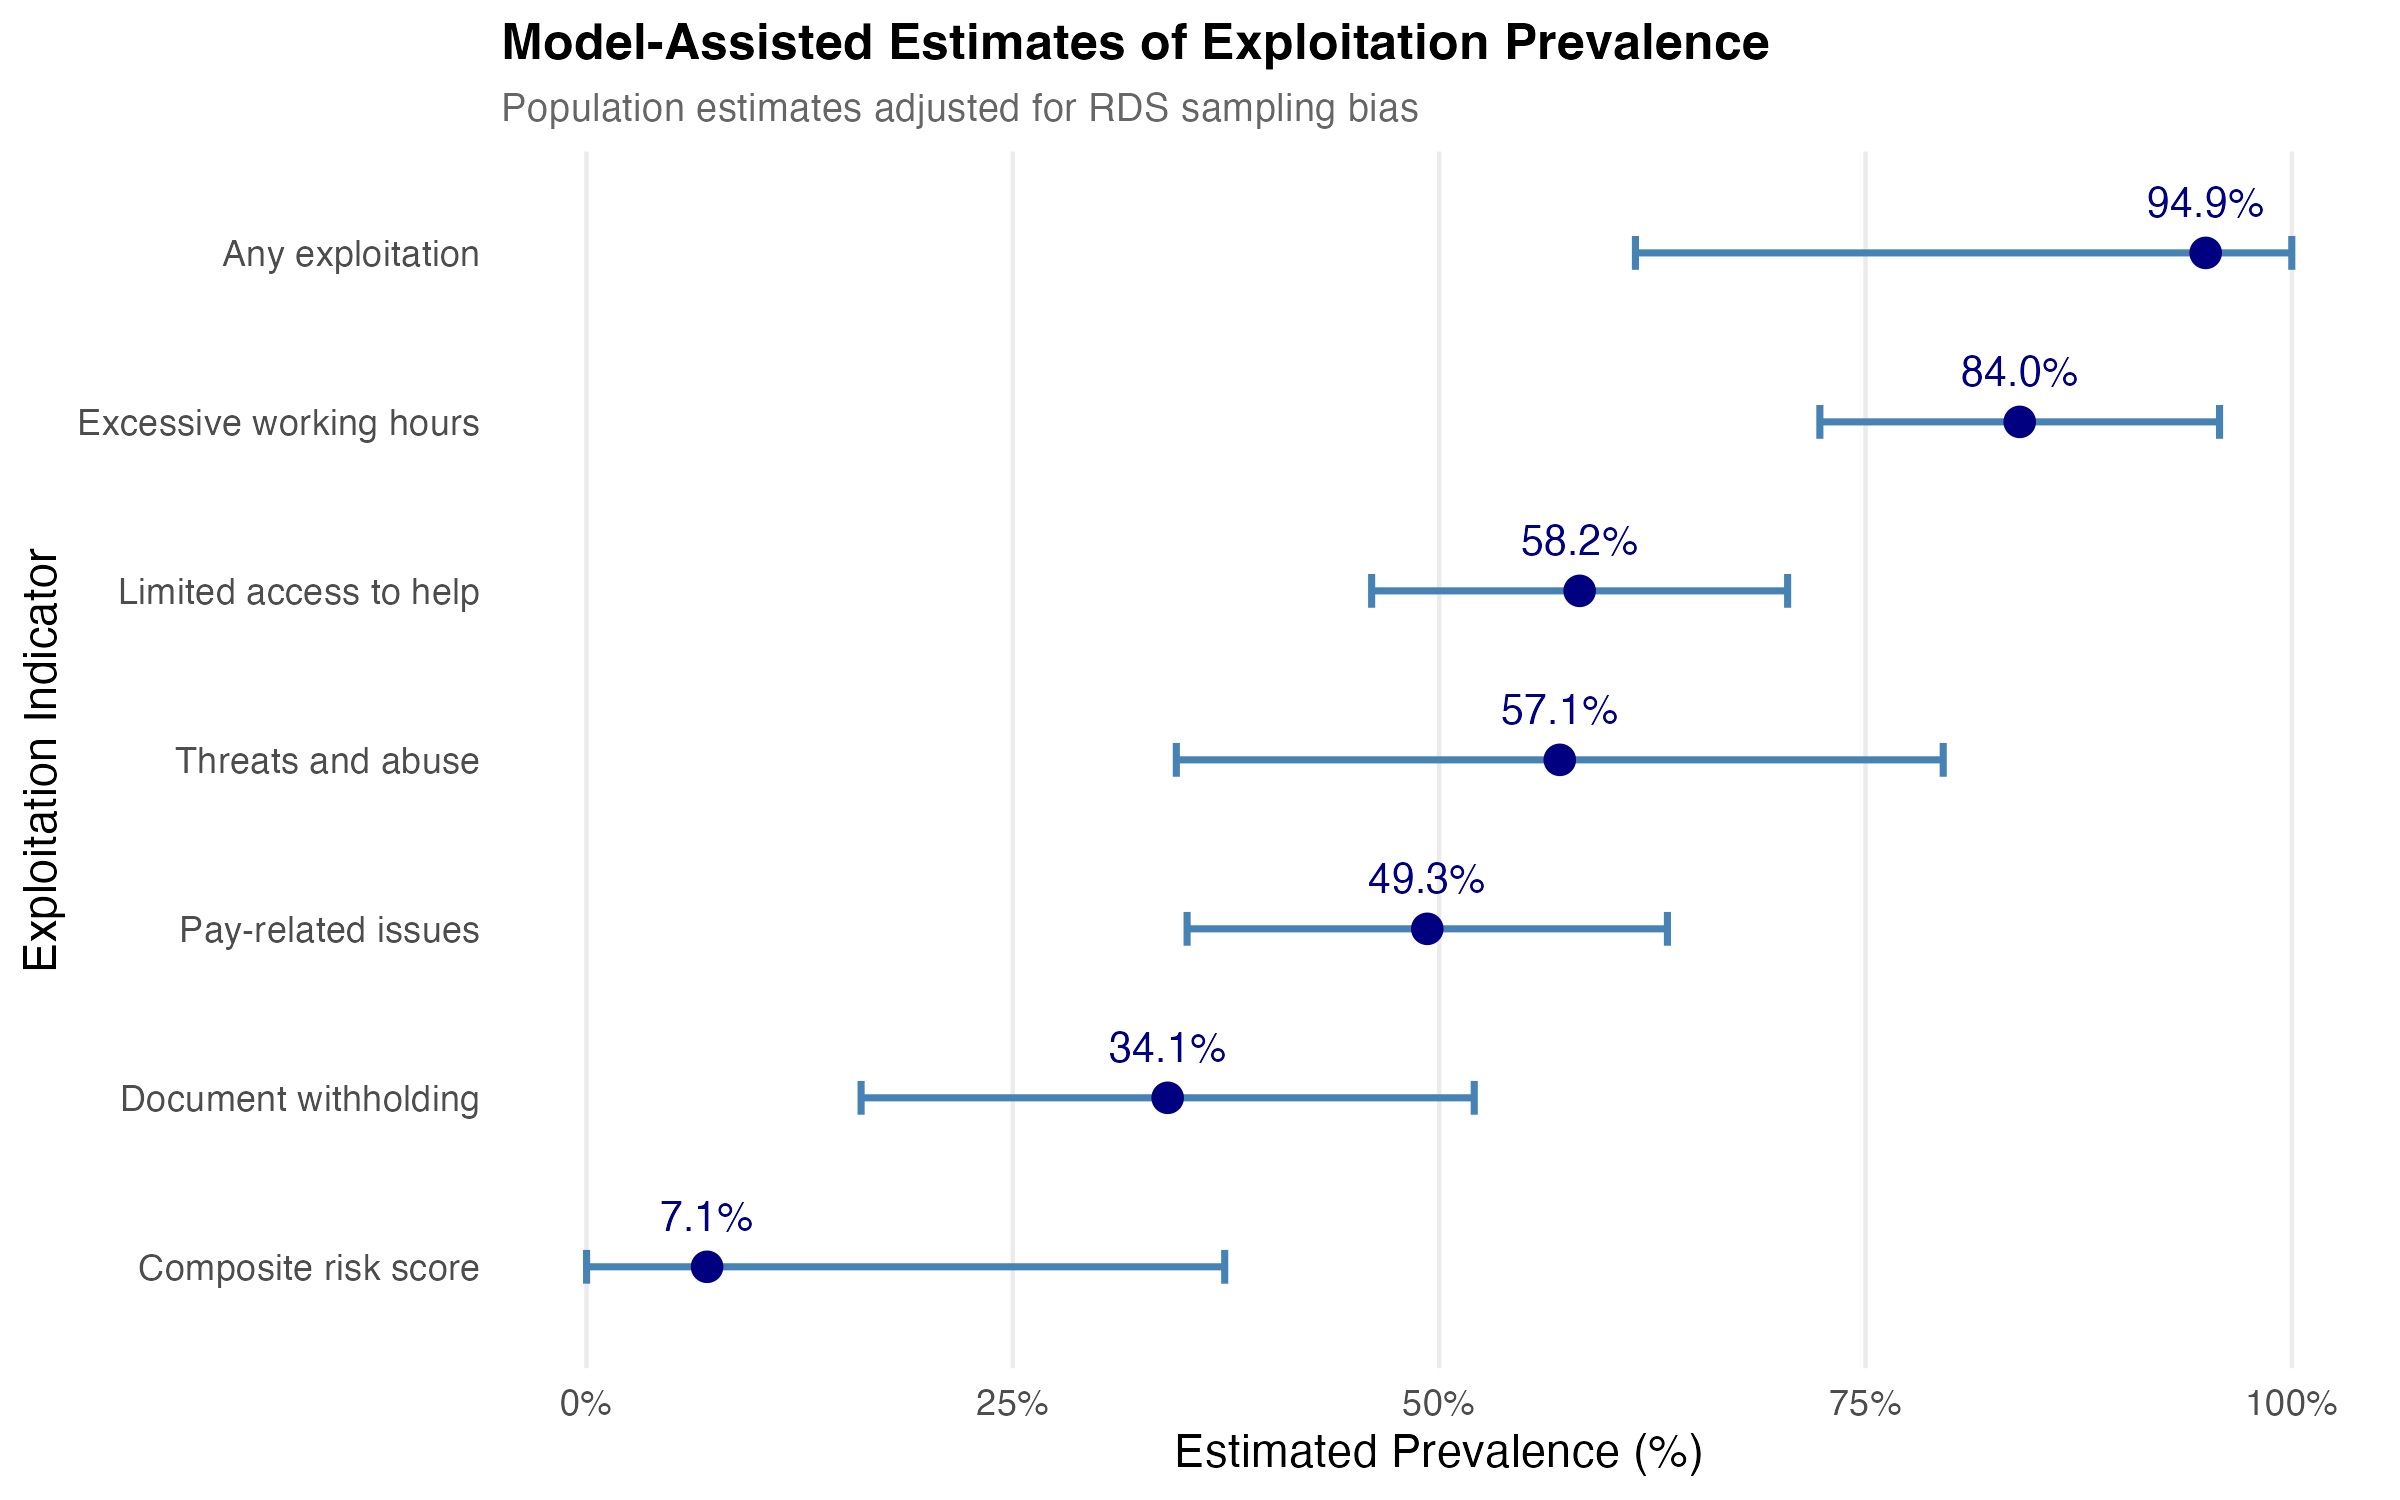
\includegraphics[width=6in,height=\textheight,keepaspectratio]{figures/fig4_ma_binary.png}

}

\caption{\label{fig-ma-binary}Model-Assisted Estimates of Exploitation
Prevalence. Population prevalence estimates with 95\% credible intervals
for each exploitation indicator, ordered by prevalence magnitude.
Posterior intervals are from Bayesian Model-Assisted inference
\autocite{gile15-network} at N=50,000 with seed.selection=`degree'.
Source: Authors' own work.}

\end{figure}%

\subsection{Supporting Estimates and Method
Comparison}\label{sec-supporting-estimates}

Three additional families of estimates are reported in full in the
Appendix (Section D) for transparency and robustness: (a) The five
Bayesian Model-Assisted (MA-RDS) posterior means (Appendix Table D.1)
range from 34.1\% for document withholding to 84.0\% for excessive
working hours, reproducing the RDS-SS ordering in
Table~\ref{tbl-preferred-estimates}. (b) Direct comparison of RDS-I and
RDS-SS estimators for each indicator with per-method bootstrap 95\% CIs
(Appendix Table D.3); RDS-I runs systematically higher than RDS-SS by
5--15 percentage points, consistent with the standard finding that RDS-I
is sensitive to seed dependence and performs poorly at the small sample
sizes and shallow chain depths characteristic of our design
(Section~\ref{sec-rds-diagnostics}). (c) NSUM under the three discrete
adjustment-factor tiers (Unadjusted, Moderate, Conservative; Appendix
Table D.4), presented for direct comparison with the discrete-tier NSUM
literature. The substantive headline NSUM result is the
continuous-\(\tau\) sweep reported in Section~\ref{sec-sensitivity}.

\subsection{Sensitivity and Robustness}\label{sec-sensitivity}

Three sensitivity analyses are reported in full in the Appendix. First,
the continuous-\(\tau\) NSUM sweep (Appendix Figure D.4) shows MBSU
prevalence monotonically increasing as \(\tau\) decreases; the increase
is modest across the plausible range \(\tau \in [0.7, 1.0]\) and
substantial only at low \(\tau \le 0.5\). This continuous picture
supersedes the discrete-tier comparison
(Section~\ref{sec-supporting-estimates}) for substantive inference about
how visibility assumptions affect estimates.

Second, the MA-RDS seed-selection sensitivity (Appendix Figure D.1)
shows that the Bayesian MA posterior estimates are insensitive to the
choice of seed-selection method (degree, random, sample) at our sample
size -- different chains converge to the same posterior, confirming
model robustness to initialisation.

Third, cross-indicator and cross-method consistency: across the five
indicators and the four main estimators (RDS-I, RDS-SS, MA-RDS, MBSU
NSUM Moderate), the rank-ordering of indicators by prevalence is stable.
Excessive working hours is consistently highest, followed by threats and
abuse and pay-related issues, with document withholding the lowest.
Absolute prevalence levels vary by method but the substantive picture --
which exploitation behaviours are most common, which least -- does not.

\section{Discussion}\label{sec-discussion}

\subsection{Summary of Findings}\label{sec-summary}

Across five ILO-aligned binary indicators measured on a
respondent-driven sample of 85 UK migrant domestic workers, RDS-SS
Horvitz-Thompson prevalence estimates range from 35.4\% for document
withholding (95\% CI 21.1--49.8\%) to 84.2\% for excessive working hours
(95\% CI 72.2--93.6\%); a composite continuous risk index covering all
eleven indicator dimensions gives an estimated mean exploitation
intensity of 37.0\% (95\% CI 30.9--44.0\%). MBSU Moderate NSUM estimates
of the same five binary indicators range from 1.08\% (document
withholding) to 2.98\% (excessive hours), an order-of-magnitude lower
than the RDS-SS figures. The within-method ordering of indicators is
consistent across methods: excessive working hours always highest,
followed by threats and abuse and pay-related issues, with document
withholding always lowest. This consistency, alongside the
order-of-magnitude gap between ego-based (RDS) and alter-based (NSUM)
estimates, is the central empirical finding of the paper. The remainder
of this section interprets both the absolute estimates and the
inter-method divergence.

\subsection{Methodological Reflections and
Contributions}\label{sec-contributions}

This paper makes two contributions to the measurement of modern slavery
among hidden populations. First, we apply RDS and NSUM to the same
matched survey instrument in what is, to our knowledge, among the first
applications of this dual design in any developed-economy setting for
the measurement of forced-labour and modern-slavery indicators; the
design supports direct comparison of ego-based and alter-based estimates
on a like-for-like indicator set without claiming they target the same
population quantity (Section~\ref{sec-estimation-framework},
Table~\ref{tbl-estimands}). Second, we operationalise modern slavery as
a graded formative indicator framework rather than a binary condition,
supporting both indicator-level prevalence estimates and an
eleven-indicator formative additive composite risk index for ordinal
severity gradation.

The combined contributions are: (i) operationalising exploitation both
as a five-indicator binary set (Section~\ref{sec-binary-results}) and as
a formative additive composite spanning all eleven ILO categories
(Section~\ref{sec-composite-results}); (ii) applying RDS and NSUM to the
same instrument, exposing the visibility gradient where the two methods
diverge (Section~\ref{sec-divergence}); (iii) implementing a three-step
bootstrap procedure for NSUM that resamples respondents, alters, and
exploitation classifications in succession; and (iv) demonstrating
feasibility in a stigmatised and under-researched population mediated by
civil-society partners, with the methodology generalisable to other
hidden populations relevant to SDG 8.7 monitoring
(Section~\ref{sec-policy}).

The paper's measurement strategy can be evaluated against five
validation channels. Content validity rests on anchoring the indicator
set in the ILO framework of forced labour
\autocite*{ILO11-indicators,hard24-ilo,int25-ilo}, with the
indicator-to-survey-question mapping in
Table~\ref{tbl-indicator-mapping}. Face validity rests on co-development
of the survey instrument with the three participating civil-society
organisations (Kalayaan, Voice of Domestic Workers, LAWRS), whose
case-work practice informed item wording. Convergent validity rests on
the reproduction of the within-method indicator ordering across four
methodologically unrelated estimators (Section~\ref{sec-sensitivity}).
Robustness rests on the composite-risk ranking being essentially
weight-invariant under ±50\% perturbation (Spearman \(\rho\) = 0.992
ρ=0.992; Section~\ref{sec-weights-sensitivity}) and on the headline NSUM
estimates being reported as a continuous function of \(\tau\) rather
than a single point. Limitation: the strategy does not yet include
external validation against administrative sources (NRM referrals,
employment-tribunal records) --- the natural next step for the broader
SDG 8.7 monitoring architecture (Section~\ref{sec-policy}).

\subsection{The RDS--NSUM Divergence as
Diagnostic}\label{sec-divergence}

Two related concerns are taken up here: that the reported prevalence
estimates span a wide range, and that the sample size (n = 85) is small
for population-level inference. The apparent ``wide range'' reflects
three conceptually distinct sources of dispersion, each carrying
different epistemic weight. Sample size operates through only one of
these three sources, and on that source \(n=85\) is competitive for
hidden-population designs.

\emph{Across-indicator variation.} Within any single method, prevalence
varies substantially across the five indicators -- under RDS-SS, from
35.4\% (document withholding) to 84.2\% (excessive working hours), a
49-percentage-point spread. This is a substantive finding, not noise:
severe forms of coercion (document confiscation, an ILO strong indicator
in \textcite{hard24-ilo}) are less common in this population than less
severe forms of abuse (excessive hours, an ILO medium indicator). The
ordering is interpretable, matches the ILO severity ordering documented
in the ILO survey-guidelines handbook \autocite{hard24-ilo}, and is
reproduced across methods. Collapsing this ordering into a single ``wide
range'' headline obscures what is arguably the paper's most
policy-relevant finding: different exploitation behaviours have
meaningfully different population frequencies.

\emph{Across-method variation.} For any single indicator, RDS and NSUM
estimates differ by roughly an order of magnitude: document withholding
35.4\% (RDS-SS) versus 1.08\% (MBSU Moderate); excessive hours 84.2\%
versus 2.98\%. This is the visibility-gradient diagnostic at the centre
of the paper's contribution: ego-based RDS asks what happened to you,
alter-based NSUM asks what you can see happening to others, and the two
answer related but different questions for behaviours that occur behind
closed doors. The gap is consistent with a visibility gradient -- some
exploitation behaviours are readily observable by peers, others remain
concealed within the household. We are cautious not to claim that the
gap \emph{quantifies} visibility, because the divergence also reflects
differences in estimand (Table~\ref{tbl-estimands}), sampling frame,
transmission bias, and the unknown true-positive rate \(\tau\) (which
the continuous-\(\tau\) sweep in the Appendix makes explicit). Reporting
RDS and NSUM side-by-side (Table~\ref{tbl-preferred-estimates}) is the
paper's design choice precisely because the gap is interpretable as
diagnostic evidence rather than as a single estimate of a single
quantity.

\emph{Within-method, within-indicator sampling variation.} This is the
only source that is irreducibly statistical uncertainty in the
conventional sense, captured by bootstrap confidence intervals. RDS-SS
within-indicator CIs span 21--30 percentage points; MBSU Moderate
within-indicator CIs span 1--4 percentage points. A residual
NSUM-specific component comes from the unknown \(\tau\), reported as the
continuous-\(\tau\) sweep in the Appendix (Section D.5, Figure D.4)
rather than as a single point. Sample size operates through this third
channel and only this third channel: more respondents would narrow the
bootstrap CIs but would not narrow the across-indicator hierarchy (which
is real) or the across-method gap (which is the diagnostic finding).

Three further observations support the visibility-gradient
interpretation. The gap is largest for indicators we would expect to be
least visible (document withholding, ego/alter ratio 33\(\times\)) and
smaller for more visible indicators (excessive hours: ratio
28\(\times\)). The within-method ordering of indicators is stable across
methodologically unrelated estimators -- a robustness signal that
justifies treating the indicators as distinct gradations of severity
even where absolute levels differ. And the direction of the bias matches
the NSUM transmission-bias literature
\autocite{kill98-social,malt15-estimating,feeh16-generalizing}, which
documents systematic alter under-reporting for stigmatised traits, often
of an order of magnitude.

On sample size: n = 85 is small by household-survey standards but
competitive for hidden-population studies (published RDS applications
operate at 100--300; UK domestic-worker NGO samples are typically
smaller and not network-recruited). The dual ego/alter design extracts
more information per respondent than a household survey, yielding 170
indicator measurements per ILO category once both reports are counted
before any network-weighting amplification. Chain depth is shallower
than the RDS design envisaged (Section~\ref{sec-rds-diagnostics}); a
longer field period would help in future replications.

\subsection{Generalisability and Indicator
Coverage}\label{sec-generalisability}

One may reasonably question whether estimates from a single
civil-society-mediated sample can support population-level claims, and
whether the five indicators we measure capture the full ILO conceptual
space. Both are valid concerns and both warrant qualification of the
paper's claims rather than retreat from them.

On generalisability: the sample is drawn from two London-based
civil-society networks (Kalayaan and the Latin American Women's Rights
Service) and is not representative of all UK migrant domestic workers,
much less all hidden populations relevant to SDG 8.7. Demographics skew
Filipino and Latinx, omitting substantial South Asian, East African, and
Eastern European communities not reached by the participating networks.
What the paper demonstrates is methodological feasibility on a hard
realistic case and a set of specific estimates for that sample; the
methodology generalises but the specific prevalence numbers should not
be extrapolated beyond this sample.

On indicator coverage: the five binary indicators bundle nine of the
eleven ILO categories (Section~\ref{sec-survey-instrument},
Table~\ref{tbl-indicator-mapping}) --- threats and abuse combines two
ILO categories (intimidation/threats and physical and sexual violence),
pay-related issues combines two (wage withholding and debt bondage),
limited access to help combines two (restriction of movement and
isolation), document withholding and excessive working hours each map to
a single ILO category, and threats and abuse also captures part of ILO
Category 10 (abusive working and living conditions) through Q48.

Putting these qualifications together, what does this design licence the
paper to claim? The four estimators (RDS-SS, MA-RDS, MBSU Moderate NSUM,
the composite risk index) each yield point estimates, but each targets a
\emph{different} population quantity (Table~\ref{tbl-estimands}):
own-experience prevalence, network-visible prevalence, and severity
score. No single estimate is identified \emph{as} `the prevalence of
forced labour among UK domestic workers', because that label spans both
ego-based and alter-based quantities at once. If RDS over-samples
respondents with first-hand experience and NSUM under-detects concealed
exploitation, the true prevalence for any given indicator plausibly lies
between the two reports -- but the precise location depends on
assumptions about visibility, sampling, and reporting that the data
cannot pin down. We treat this as a working hypothesis, not an
identification result. The design does licence (a) a conservative
reference scenario under the stated MBSU assumptions (MBSU Moderate,
\(\delta = 0.9\), \(\tau = 0.85\), sits on the conservative side of the
continuous-\(\tau\) sweep in Section~\ref{sec-sensitivity}); (b) a
credible characterisation of relative incidence (from RDS) and the
indicator severity hierarchy (from cross-method robustness); and (c) a
visibility diagnostic for network-mediated outreach
(Section~\ref{sec-policy}).

\subsection{Composite Risk Index: Construction and Weight
Sensitivity}\label{sec-weights-sensitivity}

A further question is whether the composite risk index is sensitive to
the specific weights on its eleven sub-indicators (already documented in
Section~\ref{sec-survey-instrument} and the Appendix, Section A). We
address this with a weight-perturbation sensitivity analysis: each
weight was multiplied by an independent uniform factor in \([0.5, 1.5]\)
(i.e., \(\pm 50\%\) perturbation), the composite was recomputed under
the perturbed weights, and the resulting respondent ranking was compared
to baseline. We repeated this for 5,000 independent perturbations.

The ranking of respondents by composite-risk is essentially
weight-invariant. Mean Spearman rank correlation between the perturbed
and baseline composites was \(\rho = 0.992\) (95\% range across
perturbations: 0.985--0.997), with the worst-case \(\rho\) across all
5,000 draws being 0.974. The 97.5\% interval of perturbed composites
that fell in the same top quartile as the baseline composite was
92--100\%, with a mean of 97.5\%. Even under a more aggressive ±75\%
perturbation, Spearman \(\rho\) remained above 0.944 in the worst case
across 5,000 draws and the top-quartile preservation averaged 94.4\%. We
conclude that the substantive conclusions of the composite-risk analysis
-- which respondents are at highest risk, the population mean of 37.0\%,
and the rank-ordering used for downstream analyses -- do not depend on
the specific weighting choice within any plausible alternative
parameterisation. Full perturbation results are reported in the
Appendix.

\subsection{Policy Implications and SDG 8.7
Monitoring}\label{sec-policy}

The dual RDS--NSUM design and the visibility-gradient diagnostic are
themselves policy-useful outputs for SDG 8.7 monitoring. Target 8.7
commits signatory states to ``take immediate and effective measures to
eradicate forced labour, end modern slavery and human trafficking'' by
2030, with monitoring requiring credible prevalence estimation for
populations largely invisible to official statistics. The methodology
demonstrated here -- matched ego-alter instruments fielded through
civil-society partnerships, estimated with parallel RDS and NSUM
frameworks, and reported with explicit visibility-adjustment sensitivity
-- is replicable for other hidden populations relevant to 8.7 monitoring
(undocumented agricultural workers, sex workers, kafala-system
migrants). The specific numerical estimates here apply only to UK
migrant domestic workers; the design is the contribution.

The visibility-gradient diagnostic also has direct programme-design
implications. Network-mediated outreach (peer referral, civil-society
partnership, warm handover) can only reach behaviours visible across
network ties. Our findings suggest excessive working hours is
well-suited to such outreach (small ego--alter gap), whereas document
withholding is largely invisible across ties (largest gap) and will
require different designs -- embassy or institutional intake screening
rather than peer outreach. The dual-method design therefore not only
estimates prevalence but also helps calibrate identification strategy to
the visibility profile of the behaviour.

Future work should extend the methodology to web-RDS at scale and
integrate with administrative data sources (NRM referrals, immigration
enforcement data subject to firewall safeguards, employment-tribunal
records) for triangulation against complementary data streams.

\section{Conclusion}\label{sec-conclusion}

This paper applies respondent-driven sampling and the network scale-up
method to the same matched survey instrument --- among the first such
applications in any developed-economy study of forced-labour and
modern-slavery indicators --- using a sample of 85 UK migrant domestic
workers recruited through three civil-society partnerships. The paper's
broader contribution is best read as developing and demonstrating a
defensible social-indicator measurement strategy for hidden-population
exploitation rather than as producing a definitive national prevalence
estimate. Specifically, the dual RDS--NSUM design produces two
complementary estimands; where they diverge, the gap is diagnostic
evidence about the visibility gradient of exploitation behaviours within
workers' personal networks. Second, we operationalise modern slavery as
a graded formative indicator framework rather than a binary condition,
supporting both indicator-level prevalence estimates and a continuous
formative additive composite risk index that gives equal weight to each
of the ILO's eleven indicators of forced labour and is organised for
reporting by the ILO's medium/strong severity ordering
\autocite{hard24-ilo}.

The central empirical finding is the order-of-magnitude gap between
ego-based (RDS) and alter-based (NSUM) estimates: for document
withholding, RDS-SS estimates 35.4\% prevalence vs MBSU Moderate NSUM
1.08\%; for excessive working hours, 84.2\% vs 2.98\%. The gap is
consistent with a visibility gradient across exploitation behaviours and
provides diagnostic evidence about which behaviours are observable
across network ties and which are not; it also reflects differences in
estimand, sampling frame, and transmission bias
(Section~\ref{sec-divergence}). The policy implication is that
network-mediated outreach can credibly reach exploitation behaviours
visible across ties but requires complementary designs for those that
are not (Section~\ref{sec-policy}).

The dual-method design demonstrated here is replicable. The matched
ego-alter survey instrument, parallel RDS and NSUM estimation framework,
and explicit visibility-adjustment sensitivity reporting can be applied
to other hidden populations relevant to SDG Target 8.7 monitoring ---
undocumented agricultural workers, sex workers, kafala-system migrants
--- and any population for which official statistics are silent.

\section{Declarations}\label{sec-declarations}

\textbf{Funding.} CE received funding from the University of Nottingham
under its Nottingham Research Fellowship scheme.

\textbf{Competing interests.} The authors have no competing interests to
declare.

\textbf{Ethics approval and consent to participate.} The data collection
that underpins the analysis presented in this paper was given favourable
ethical approval by the lead author's School Research Ethics Committee
in January 2023 (Ethics Review Application number 202223021). All
participants were informed about the aims of the study, provided
informed consent, and were assured that participation was voluntary and
confidential.

\textbf{Data availability.} Anonymised respondent-level data and all
analysis code are available at the project's Open Science Framework
mirror:
\url{https://osf.io/vf5yb/overview?view_only=becc2db3b49c4b258015b648867bf208}.
The underlying GitHub repository is currently private and will be made
public on acceptance.

\textbf{Use of large language models.} The authors used a large language
model assistant (Anthropic Claude) for textual editing and for
code-review support during R script development. All final analysis
decisions, statistical interpretations, and prose are the authors' own.
No generative models were used to simulate, augment, or fabricate data.
This disclosure follows the Springer Nature editorial guidance on the
use of generative AI tools in scholarly work.

\textbf{Authors' contributions.} CE designed and collected data; SM
performed analysis. Both contributed to the writing of the document.

\newpage

\section*{References}\label{references}
\addcontentsline{toc}{section}{References}

\printbibliography[heading=none]





\end{document}
